
\documentclass[journal,article,accept,oneauthors,pdftex,10pt,a4paper]{mdpi} 

\firstpage{1} 
\makeatletter 
\setcounter{page}{\@firstpage} 
\makeatother 
\articlenumber{x}
\doinum{10.3390/------}
\pubvolume{xx}
\pubyear{2016}
\copyrightyear{2016}
%\externaleditor{Academic Editor: name}
%\history{Received: date; Accepted: date; Published: date}

\usepackage{pgf}
\usepackage{tikz}
\usepackage[utf8]{inputenc}
\usetikzlibrary{arrows,automata}
\usetikzlibrary{positioning}
\usepackage{float}
\usepackage{makecell}
\usepackage{array,multirow,graphicx}
\usepackage{slashbox}
\usepackage{hhline}
\usepackage{listings} 
\usepackage{pgfplots}
\usepackage{mathabx}

\tikzset{
    state/.style={
           rectangle,
           rounded corners,
           draw=black, very thick,
           minimum height=2em,
           inner sep=2pt,
           text centered,
           },
}
\lstset{language=Python}
\pgfplotsset{width=14.5cm,compat=1.9}

%------------------------------------------------------------------
% The following line should be uncommented if the LaTeX file is uploaded to arXiv.org
%\pdfoutput=1

%=================================================================
% Add packages and commands here. The following packages are loaded in our class file: fontenc, calc, indentfirst, fancyhdr, graphicx, lastpage, ifthen, lineno, float, amsmath, setspace, enumitem, mathpazo, booktabs, titlesec, etoolbox, amsthm, hyphenat, natbib, hyperref, footmisc, geometry, caption, url, mdframed

%=================================================================
%% Please use the following mathematics environments: Theorem, Lemma, Corollary, Proposition, Characterization, Property, Problem, Example, ExamplesandDefinitions, Remark, Definition
%% For proofs, please use the proof environment (the amsthm package is loaded by the MDPI class).

%=================================================================
% Full title of the paper (Capitalized)
\Title{A Numerical Solver for a new form of arbitary Markov-Decision-Evolutionary-Games}

% If this is an expanded version of a conference paper, please cite it here: enter the full citation of your conference paper, and add $^\dagger$ in the end of the title of this article.
%\conference{}

% Authors, for the paper (add full first names)
\Author{Mark Burgess}
% Authors, for metadata in PDF
\AuthorNames{Mark Burgess}

% Affiliations / Addresses (Add [1] after \address if there is only one affiliation.)
\address{%
 \quad Research School of Computer Science, The Australian National University, Canberra, ACT 0200, Australia; markburgess1989@gmail.com}


% Simple summary
%\simplesumm{}

% Abstract (Do not use inserted blank lines, i.e. \\) 
\abstract{We introduce a structure for the presentation of a new type of Markov-Decision-Evolutionary-Games (MDEG) conductive to a new computational technique to determine Evolutionary Stable Strategies.
The treatment incorporates arbitary numbers of states with arbitary decisions between states and can incorporate non-linear transitions (as dependant on endogenous variables) between states in the game. The software presented is designed to be extensible to the purpose of analysing the distribution of Evolutionary Stable Strategies across relevant sets of exogenous variables.\\
Following the example of others we introduce a statefull Hawk-Dove MDEG and solve for its Evolutionary Stable Strategies; we compare computed results with thoes attained via analysis and also via monty-carlo methods as example of the working system. We then move on to examine a significantly more complex game examining the hypothetical relationship between Paternal Uncertainty and Paternal investment in mating dynamics. We finish with philosophical remarks on the role and use of this and other similar software.}

% Keywords
\keyword{Evolutionary stable strategies (ESS); Markov decision evolutionary games (MDEG); Hawk-Dove game; Evolutionary dynamics; Evolutionary Game Theory;}

%\setcounter{secnumdepth}{4}
%%%%%%%%%%%%%%%%%%%%%%%%%%%%%%%%%%%%%%%%%%
\begin{document}

\section{Introduction}

The merging of Game Theory and Evolutionary Concepts is often credited to John Maynard Smith and George R. Price \cite{maynard}\cite{maynard2} specifically the introduction of the concept of Evolutionary Stable Strategy (ESS) with basic games and replicator dynamics to illustrate evolution with the concepts of game theory.
Sometimes the analysis of evolutionary games is used as grounds to explain various features of the biological world (eg. where tit-for-tat strategy superiority is sometimes thought to be indicative for the emergence of reciprocity in species\cite{titfortat}).
ESS stategies are held to be attractors of the process of evolution:
\begin{quote}"The presence of such [ESS] users then. in whatever small numbers initially, intuitively would suggest that an eventual stable equilibrium would occur if for no other reason than because the numbers of ESS users would steadily increase indefinitely otherwise, and in that manner alone force the population to the ESS ...."\cite{ess1}\end{quote}
Some go so far as to say that:
\begin{quote}"[ESS] has become widely incorporated into our thinking about biological phenomena.. a valuable point of attack on a surprising number of questions about the practice of theoretical biology"\cite{ess1}\end{quote}
Yet ESS itself is a precisely defined mathematical concept existing in the context of specific game theory analysis of populations and have precise mathematical definition in terms of the expectations of the strategy payoffs.
J\"orgen Weibull gives outline and particular restrictions on the concept's applicability: 
\begin{quote}"Suppose that individuals are taken from a large population to play a symmetric two-person game, and suppose that all individuals are genetically or otherwise 'programmed' to play a certain pure or mixed strategy in this game. Now inject a small population share of individuals who are likewise programmed to play some other pure or mixed strategy. The incumbent strategy is said to be 'Evolutionary Stable' if for each such mutant strategy, there exists a positive invasion barrier such that if the population share of individuals playing the mutant strategy falls below this barrier then the incumbent strategy earns a higher payoff than the mutant strategy"\cite{weibull}\end{quote}

Particular attention must be drawn to the representative link between the game's assigned payoffs and biological fitness:
\begin{quote}"[ESS] is focused on symmetric pair-wise interractions within a single large population. In particular it does not deal with interactions that take place between more than two individuals at a time. Moreover the criterion of evolutionary stability refers implicitly to a close connection between the payoffs in the game and the spreading of a strategy in a population. The payoffs in the game are supposed to represent the gain in biological fitness or gain in reproductive value from the interaction in question. ... and evolutionary stability is a robustness test against a \textit{single} mutation at a time"\cite{weibull}\end{quote}

It is noted that fitness is a concept that is suprisingly nuanced and held to be quite central to evolutionary theory.\cite{sep-fitness} Among many things it can not only refers to a biological individual's probably having more immediate offspring over lifespan than a less 'fitter' individual, but also of thoes decendants themself potentially having more offspring, and their decendants and so on. Another note, is that fitness is often held to be relative to the environment of the individual including the context of its peers and/or competitors.
In this paper we work with a notion of the fitness of an individual as the expected growth-rate of a steady-state population of such individuals in the context of particular environment and we introduce a specification of Evolutionary game design that does away with having to explicitly specify payoff values.

\subsection{The Introduction of State}

Evolutionary Game-Theory (and Classical Game-Theory) typically involves the analysis and dynamics only between player strategies but there has been work to extend this analysis to include states aswell. A particularly well established extension involves incorporation of state as position on a 'grid', such games are called 'Spacial Evolutionary Games'\cite{spacial1}. Spacial Evolutionary Games have unique and dynamic behavior\cite{spacial2} and have been used to study cooperation and reciprocity\cite{spacial3}, they have also been extended to arbitary graph structures\cite{spacial4}.
Yet more recent work has been done to generalise this incorporation of state into evolutionary games, particularly the work of Eitan Altman\cite{markov2}\cite{markov3}\cite{markov4}\cite{markov5} who introduces the concept of the Markov-Decision-Evolutionary-Game (MDEG) as:
\begin{quote}
"We consider a large population of players in which frequent interactions occur between small numbers of chosen individuals. Each interaction in which a player is involved can be described as one stage of a dynamic game. The state and actions of the players at each stage determine an immediate payoff (also called fitness in behavioral ecology) for each player as well as the transition probabilities of a controlled Markov chain associated with each player. Each player wishes to maximize its expected fitness averaged over time.
This model extends the basic evolutionary games by introducing a controlled state that characterizes each player.
The stochastic dynamic games at each interaction replace the matrix games, and the objective of maximizing the expected long-term payoff over an infinite time horizon replaces the objective of maximizing the outcome of a matrix game. Instead of a choice of a (possibly mixed) action, a player is now faced with the choice of decision rules (called strategies) that determine what actions should be chosen at a given interaction for given present and past observations."\cite{markov3}
\end{quote}
The MDEG bears and extremely close similarity of concept with the well studied Markov Decision Processes (MDP) except without the population coupling. MDPs have well known general solution methodologies such as various schemes of policy-iteration with iterative methods of refining the policy (aka strategy/decision rules) to optimum; and there are evolutionary schemes as well.\cite{markov6}
The central refinement of MDEG which we present is that rather than considering the individual's fitness to be the expected sum of game payoffs it achieves over an infinite time-horison we instead consider the fitness to be the expected growth of a steady-state population of such individuals.

\subsection{Stationary Growth}

in both MDP and MDEG one of the core structrures underlying the analysis is that of a Markov Chain/s representing states and probability of transitioning between them.
It is well established that if the set of states in a Markov chain are mutually connected (specifically that the Markov chain is ergodic) then there exists a unique steady state between the transitions called a 'steady distributon'.
The existance of such a distribution is due to the fact that Markov chains can be represented as non-negative matricies sufficient for the Perron–Frobenius theorem to yield existance and uniqueness of the positive eigenvector representing the 'stationary distribution'; such a distribution is redily calculated numerically and one simple technique is the eigenvector calculating 'power iteration' method.\cite{markov7}
A central tennent in the definition of a Markov chain is that an individual in any state must transition to some states and thus the total probability of all transitions from any state must sum to one.
This restriction is represented in the columns of the representing matrix must sum to one and thus the eigenvector corresponding to the 'steady distribution' has an eigenvalue of one.

It is important to note there are other known matricies representing probable transitions between states which relax this restriction and yet have unique steady state via the same Perron–Frobenius theorem.
A particularly well known example class of such a matricies are the Leslie Matricies used for studying the structure of populations of individuals (origionally for female individuals) transitioning between age-states.
Leslie Matricies (just like markov chain matricies) are square, and they have form:\cite{leslie}

\begin{equation*}
M=\begin{bmatrix}
    F_0 & F_1 & F_2 & F_3 & \dots  & F_{m-2} & F_{m-1} & F_m  \\
    P_0 &  0  &  0  &  0  & \dots  &    0    &  0    &  0   \\
     0  & P_1 &  0  &  0  & \dots  &    0    &  0    &  0   \\
     0  &  0  & P_2 &  0  & \dots  &    0    &  0    &  0   \\
     0  &  0  &  0  & P_3 & \dots  &    0    &  0    &  0   \\
    \vdots & \vdots & \vdots & \vdots & \ddots & \vdots & \vdots & \vdots \\
     0  &  0  &  0  &  0  & \dots  & P_{m-2} &  0    &  0   \\
     0  &  0  &  0  &  0  & \dots  &    0    & P_{m-1} & 0   \\
\end{bmatrix}
~~~0<P_x<1;~~F_x\ge0
\end{equation*}
For a column vector $n = [n_0,n_1,n_2,\dots,n_m]$ with each $n_x$ representing the number of individuals in each incremental (and evenly spaced) age-bracket within the population, with $P_x$ representing the probability of and individual in the $x$th age bracket successfully living into the $x+1$th age bracket, and $F_x$ being the expectation on the number of offspring for an individual in $x$th age bracket within the duration of the age bracket.

Application of the matrix $M$ to the column vector, $Mn$ gives the expected number of individuals in the population after the duration of one age bracket of time, and $M^2n$ the expectation individuals after two age brackets, $M^3n$ the population distribution after three, and so on.
Successive applications of the matrix eventually yeild a steady population profile between the $n_x$, and a constant exponential growth rate $\lambda$ given by the Euler–Lotka equation.
The $\lambda$ is simply the dominant and only real-positive eigenvalue of the matrix, with the steady distribution $n$ its eigenvector, that is $Mn=\lambda n$.

Although the elements in the Leslie matrix are positive and represent states and transition between, it cannot be representative of a Markov-chain because its columns dont nessisarily sum to one.
The informal summary difference is that wheras in a Markov-chain matrix the elements represent expectation of \textit{transition} between states, Leslie matrix elements represent expectation of \textit{transmission} between states (which we will term a 'transmission matrix').

It is in light of the calculation of growth rate via Leslie Matricies that we reiterate our interpretation of biological fitness - that the fitness of an individual is the expected growth of a steady-state population of such individuals.
As an example of the rationale of this interpretation: Consider a population of organisms where there is a single instance of a mutation that significantly increases expected number of offspring but leaves all the offspring (or perhaps the offspring's offspring) in a state of sterility.
It is quite intuitive to think that such a mutation would have the lowest possible fitness and would certainly die out in the process of evolution despite the fact that the organism with the mutation would have a high number of offspring and the growth-rate in number of organism may be significant. Under our interpretation the fitness of the mutant organism would be represented as a value of zero as a steady-state population of such mutants would have zero growth rate.

In what follows we derive the transmission matrix of different strategies, and evaluate the strategies growth as its fitness measure in the context of an evolutionary scheme.
Interpreting the fitness (or the payoff) to be the eigenvalue of a matrix seems to be something that is missing from literature at large and contrasts with existing literature on MDEG (and MDP) where the fitness of a mutation (or optimality of a policy respectively) is taken to be the sum of smaller fitnes/payoff values expected to achieved by following a markov-chain transition matrix.
By taking our evaluation of fitness we are freed from having to specify payoff/fitness values over-and-above specifying transmission rates, however this introduces quite subtle differences in Evolutionary-Game-Theory definitions and dynamics.

\section{An Example Game}

One of the most famous and earliest example evoltuionary games is that of Hawk-Dove\cite{maynard} which has been extended to multiple states by Eitan Altman\cite{markov5}.
A simplification of Altman's game is as follows:
\begin{center}
\fbox{\begin{minipage}{16cm}
Imagine a population of simple organisms that can occupy three distinct distinct States: Young, Agressive Adult, Passive Adult.
And that the organism's genome encodes a single probability $\gamma$ - that the Young will (if given the opportunity) mature into an Agressive Adult as opposed to a Passive one.

Imagine that in a distinct unit of time the Young of the population mature into a type of Adult, and also that the Adults die leaving Young offspring.
That a young organism suffers a static probability $C$ of encountering an adult before maturing and if encounters an Agressive Adult then has a static probability of surviving $D$ and matures into a Passive Adult, otherwise matures into an agressive Adult or passive adult depending on its genome.

That the Adults in the population of both types have offspring directly dependant on the proportion of Adults that are Agressive $p$.

Agressive adults in a population of Passive ones take all resources and have expectation of two offspring, whereas in a population of Agressive ones expend significant energy fighting for resources and have no offspring. Agressive adults will have expected offspring $2(1-p)$

Passive adults in a population of Passive adults will generally share resources and save energy by not fighting giving them $1+A$ expected offspring (where $A$ is a static number; $0<A<1$). But in a population of Agressive ones will loose resources to the Agressive Adults and have $A$ expected offspring. Passive adults will have expected offspring $1-p+A$
\end{minipage}}
\end{center}



The flow of organisms between possible states can be described as per the following Diagram:
\begin{figure}[H]
\begin{center}
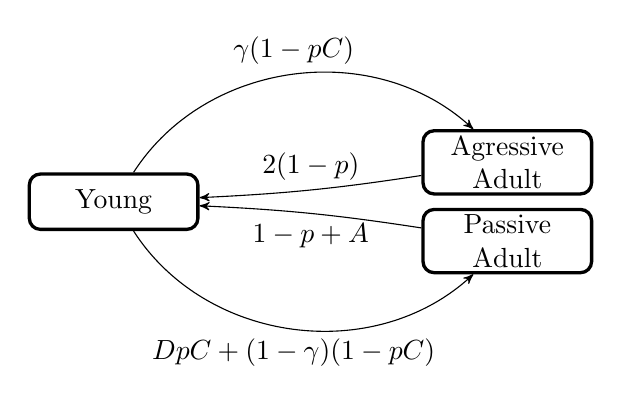
\begin{tikzpicture}[->,>=stealth']

    \node[state,anchor=center,text width=2cm]
        (Y) {Young};
    \node[state,anchor=center,text width=2cm,yshift=0.5cm,right of=Y,node distance=5.0cm]
        (A) {Agressive\\Adult};
    \node[state,anchor=center,text width=2cm,yshift=-0.5cm,right of=Y,node distance=5.0cm]
        (P) {Passive\\Adult};

    \path (Y) edge[bend left=50]  node[anchor=south,above]{$\gamma(1-pC)$} (A);
    \path (A) edge[bend left=3]   node[anchor=south,above]{$2(1-p)$} (Y);
    \path (P) edge[bend left=-3]   node[anchor=south,below]{$1-p+A$} (Y);
    \path (Y) edge[bend left=-50] node[anchor=south,below]{$DpC+(1-\gamma)(1-pC)$} (P);

\end{tikzpicture}
\end{center}
\caption{A diagram of the flow of individual organisms between states of a simple Hawk-Dove game\\$\gamma$ being genetic parameter, $p$ being proportion of Adults that are Agressive, and $A$,$D$,$C$ being game parameters}
\end{figure}
The Game can be decomposed into States and Actions in a manner resemblant of MDP:
\begin{figure}[H]
\begin{center}

\begin{tabular}{llllll}
\multicolumn{2}{l}{\multirow{2}{*}{}}      & \multicolumn{4}{c}{Actions}                                                                       \\
\multicolumn{2}{l|}{}                        & \multicolumn{1}{c|}{Young} & \multicolumn{1}{c|}{Young} & \multicolumn{1}{c|}{Aggressive} & \multicolumn{1}{c|}{Passive} \\ \cline{2-6} 
\multirow{3}{*}{\rotatebox[origin=c]{90}{\parbox[c]{1cm}{\centering State}}} 
                   & \multicolumn{1}{c|}{Young} & \multicolumn{1}{c|}{0}  & \multicolumn{1}{c|}{0}  & \multicolumn{1}{c|}{$2(1-p)$}  & \multicolumn{1}{c|}{$1-p+A$}  \\ \cline{2-6} 
                   & \multicolumn{1}{c|}{Aggressive} & \multicolumn{1}{c|}{$1-pC$}  & \multicolumn{1}{c|}{0}  & \multicolumn{1}{c|}{0}  & \multicolumn{1}{c|}{0}  \\ \cline{2-6} 
                   & \multicolumn{1}{c|}{Passive} & \multicolumn{1}{c|}{$DpC$}  & \multicolumn{1}{c|}{$DpC+1-pC$}  & \multicolumn{1}{c|}{0}  & \multicolumn{1}{c|}{0}  \\ \cline{2-6} 
\end{tabular}
\end{center}
\caption{A table showing the transmission of individuals to states in the Hawk-Dove game depending on what action is taken from what states, the genetic factor $\gamma$ is the probabilty of organism choosing the first over the second action from youth state.}
\end{figure}
Various observations can be made about this game: 
\begin{itemize}[leftmargin=*,labelsep=4mm]
\item	Where the population consists entirely of Passive Adults ($p=0$) any organism with $\gamma>0$ will have greater reproductive success and growth rate than the population and thus increase the number of Agressive Adults.
\item	Where the population consists entirely of Agressive Adults ($p=1$) any organism with $\gamma<1$ will have greater reproductive success and growth rate than the population and thus increase the number of Passive Adults.
\end{itemize}
It seems that there exists a possible evolutionary equilibrium between Passive and Agressive Adults dependant on $A$,$D$, and $C$ even if it is not so apparent.
While this particular game is simple enough that it could be reformulated as an MDEG, there are difficult questions that MDEG would obscure (eg. what proportion of the population is Young at equilibrium, between parameters $A$,$D$, and $C$).
It is also seen that the game reduces to a transmission matrix by which we can calculate the growth-rates and therefore the fitnesses of organisms (as defined by their $\gamma$ value) in the context of population $p$.
\begin{figure}[H]
$$ \lambda \begin{bmatrix}
    Y \\
    A \\
    P \\
\end{bmatrix} = \begin{bmatrix}
    0 & 2(1-p) & 1-p+A & \\
    \gamma(1-pC) & 0 & 0  & \\
     DpC+(1-\gamma)(1-pC)  & 0 & 0  & \\
\end{bmatrix}\begin{bmatrix}
    Y \\
    A \\
    P \\
\end{bmatrix} $$
\caption{The transmission matrix of the Hawk-Dove game, where vector $[Y,A,P]$ is steady state proportion of individuals with genetic factor $\gamma$ in context of population $p$}
\end{figure}
We will return to this game later where we calculate the equilibrium outcome analytically, and also via software simulation and compare our results to Monty-Carlo methods.

\section{The new Evolutionary Game}

There are three essential elements to the evolutionary game - $S$,$A$,$T$:
\begin{itemize}[leftmargin=*,labelsep=4mm]
\item	$S$ is a finite set of states
\item	$A_s$ is finite set of actions available from a state $s\in S$; $A=\cup_s A_s$; $A_s \ne \emptyset$
\item	$T_s(a,P)$ is the transmission to state $s\in S$ when action $a\in A$ is taken in the context of $P$; $T_s\ge 0$\\ where $P(s)$ is the proportion of the population in state $s\in S$; $P(s)\ge 0$; $\sum_{s\in S}P(s)=1$
\end{itemize}
We consider the game with the restriction that there is at-least one action per state even if it transmitts zero to all states.

\subsection{Strategy Sets}

In the game we consider the potential probability of taking 'what actions across what states' as the defining concept of a strategy.
And in accordance with standard game-theory jargon, we define a map from states to actions as defining a 'pure' strategy and a probability distribution across 'pure' strategies as a 'mixed' strategy.
\textit{Ipso facto} a strategy is thus considered as a random function $Z: S \rightarrow A$, with the obvious constraint $Z(s)\in A_s$. We define set of all pure strategies to be $\theta$, and all mixed strategies to be $\Theta$.

If we enumerate the states of the game $S=(s_0,s_1,s_2,\dots,s_m)$ and we take the expectation of transmission as a result of playing a strategy $Z$, then $E[T_{s_j}(Z(s_i),P)]$ ($E[\cdot]$ is expectation) is the transmission from state $i$ to $j$ and thus our transmission matrix is:
$$M(Z,P)_{i,j}=E[T_{s_j}(Z(s_i),P)]$$

Matrix $M(Z,P)_{i,j}$ is the transmission matrix between indexed states $i$ to $j$ and so its positive real eigenvalue is the growth-rate and fitness/payoff of strategy $Z$ in context of population $P$.\footnote{Note should be made that the rather general matrix $M(Z,P)$ occasionally may not satisfy the conditions of the Perron–Frobenius theorem (that the transmissions between states not constitute an 'ergodic' set) and thus not have a positive-eigenvalue that is nessisarily unique, though it will nessisarily have a largest positive eigenvalue (as for instance, found by power-iterations) which is sufficient for our purposes.}

\subsection{Evolutionary Stability}

It is particularly important to note that stability with regards to an evolutionary process is intrinsically linked with the dynamics (however defined) of the process itself.
A prominant feature of Evolutionary Game theory literature is the modelling of the evolutionary dynamics against game-theory payoffs via the replicator equation:
$$ \dot{x}_i = x_i ( \pi_i - \langle\pi\rangle)$$
where $x_i$ is the proportion of the population playing strategy $i$ and $\pi_i$ is the game payoff for playing $i$ against the population, whos average payoff is $\langle\pi\rangle$.
The replicator equation is supported as a model for evolutionary dynamics for various reasons, not limited to its connection to evolutionary dynamics of (two-player) interactions between individuals of finite populations.
Particularly that dynamics of the replicator equation is the large-population-limit of finite-games such as the Moran or Wright-Fisher processes.\cite{stochastic1}\cite{stochastic2} And all of which have a straightforward biological interpretation in terms of competition between dominant genes\cite{replicator1}.

The evolutionary stable points of an evolutionary process are not nessisarily identical with points ESS, even under the replicator equation.\cite{replicator1}
Furthermore Nowak spells out that incorporating even a mutation term into the standard replicator equation changes the dynamics of the process and distinctly warps the position of Evolutionary Stable points from thoes that might otherwise be ESS.\cite{nowak}

Finding points of stability with regard to a specified evolutionary process constrasts with the most established process of finding ESS points.
ESS was origionally defined by Maynard Smith\cite{maynard}\cite{maynard2} to be a robust quality of payoffs of particular sets of strategies in the symmetric two-person game in which the population was to mutually participate:
\begin{quote}"[ESS] is focused on symmetric pair-wise interractions within a single large population. In particular it does not deal with interactions that take place between more than two individuals at a time ... and evolutionary stability is a robustness test against a \textit{single} mutation at a time"\cite{weibull}\end{quote}
And is sometimes defined as\cite{replicator1}\cite{weibull}: a strategy $p*$ is ESS iff for all other strategies $p$:
\begin{enumerate}[leftmargin=*,labelsep=3mm]
\item	$\pi(p,p*)\le \pi(p*,p*)$
\item	$\pi(p*,p)>\pi(p,p)$ if $\pi(p,p*) = \pi(p*,p*)$
\end{enumerate}
where $\pi(x,y)$ is the payoff (however defined) of playing strategy $x$ against population strategy $y$, note that the first of these is the critereon of weak Nash Equilibrium and thus ESS points are subset of weak Nash Equilibrium points. (we use these definitions implicitly for calculation of ESS of the above Hawk-Dove game in Appendix A)

Thus the defining critera for ESS is that it either strictly dominates other strategies or if it weakly dominates another strategy then it performs better in the context of that other strategy than it does. It is thus intuitive and expected that ESS points would often be points of evolutionary stability: "[ESS are] a strategy which, if adopted by a population in a given environment, cannot be invaded by any alternative strategy that is initially rare"\cite{gloss1}\cite{maynard}, "[the ESS] property does not explain \textit{how} a population arrives at such a strategy, Instead it asks whether, once reached, a strategy is robust to evolutionary pressures"\cite{weibull}; and thus be indicative of a stable result of an evolutionary process.

The classical definition has it as being essentail that the game and its payoff matrix be two-player and symmetrical $\pi(x,y)=\pi(y,x)$ although in certain cases this critereon has been relaxed\cite{replicator1}.
By allowing the relaxation of symmetry requirement it is possible to directly extend the critereon for ESS points to our case (where the payoff is identified with the eigenvalue of the transmission matrix of a strategy in context of an effective population strategy - which is not nessisarily symmetric) and so it is possible to find them algebraically (as we do in Appendix A).

Notwithstanding, in the case of our solver, it isnt ESS points \textit{per sei} that we are interested in, so much as points of evolutionary stability that occur as a result of a specified evolutionary process.

It is therefore quite sufficient to define the evolutionary process (be that two-player, symmetric with mutation or not) and then turn to examining its points of \textit{convergence} -and thence stability- under such a process.
So we present a scheme for specifying a general evolutionary process by which it is possible for us to computationally determine points of convergence by an iterative scheme; giving points which may be ESS depending on the particular implementation.

\subsection{Defining an Evolutionary Processes}

Even under Classical Evolutionary Game Theory the process of evolution is not nessisarily prescribed, as even the replicator equation is not mandatory.
It is generally understood that the the payoffs in the game should be postively correlated with growth-rate but exactly how is left unspecified.
Sometimes there is specified a 'growth-rate' function generalising the replicator equation $\dot{x}_i=g_i(x,t)x_i$ with the quality of having 'positivity in correlation' as known as 'payoff-monotonicity' of the growth function: $\pi(e^i,x) > \pi(e^j,x) \Leftrightarrow g_i(x,t) > g_j(x,t)$\cite{weibull} with $e^i$ being pure strategy $i$.
It is also possible to introduce other elements such as a mutation term $\dot{x}_i=g_i(x,t)x_i+\mu_i(x,t)$\cite{nowak}.
The evolutionary process in the most general form: $\dot{x}_i=h_i(x,t)$.

It is obviously possible to equate the growth function with the payoff itself $ g_i(x,t) = \pi(e^i,x)$, $~~\mu_i=0$, leaving the payoff-monotonicity condition trivial and giving replicator equation dynamics, however such an equation isnt nessisarily desirable.

Various Evolutionary Games feature instability of a global or local character, a well known example is the various class of Paper-Scissors-Rock games\cite{rockpaperscissors} (see next section) where direct applicaton of the replicator equation will not converge to a stable state under some variations, and under other variations would only converge very slowly.

Computational iterations with a time step $T$ where $dx_i=x_i(g_i(x,t)) T$ can lead to the introduction of artificial instability depending on the size of the time step (and form of $g_i(x)$) it is known that articicial instability can be ameliorated by having a sufficiently small time-step OR having a slowly decaying time-step (where $\lim_{t\rightarrow\infty}T(t)=0$, $\sum_{t=0}^\infty T(t)=\infty$).\cite{errors1}

One extreme example of such a growth function $g$ is of having equal zero growth for all strategies but the ones with the greatest payoff, and this is known as best-response incorporation and has potential to converge very quickly at the cost of being potentailly unstable.
Iterative best response incorporation has proven convergence under some strict conditions; the most notable of which is that the 'best response mapping' (the map from population state to best mutation strategy') be continuous, which in many games simply isnt so.\cite{nash1}\cite{errors1}

There is freedom and choice in the evolutionary process for various results, which will be illustrated at length in the next section.

Inspired by the example of McNamara et.al\cite{errors1} we describe a set of general growth functions $h$ by an 'error function' $R$.
$$ h_i(x,t) = \frac{R(\pi(e^i,x),\bigtimes_{j\in\theta}\pi(e^j,x))T(t)}{\sum_{k\in\theta} R(\pi(e^k,x),\bigtimes_{j\in\theta}\pi(e^j,x))} $$

In this way the error function $R$ takes in all the payoffs of the strategies in the game (that is $\bigtimes_{j\in\theta}\pi(e^j,x)$) and in light of that spectrum of payoffs returns the 'weight' of strategy of payoff $\pi(e^i,x)$.
the growth rate $h_i(x,t)$ is then the 'weighted' payoff of the strategy $e_i$ multiplied by the time decay function $T(t)$.

The iteration central to our solver is a simple forward-difference scheme on the equation $\dot{x}_i=h_i(x,t)$.
That is:

$$\boxed{x^{t+1}_i = N_t\left(x^t_i + \frac{R(\pi(e^i,x^t),\bigtimes_{j\in\theta}\pi(e^j,x^t))T(t)}{\sum_{k\in\theta} R(\pi(e^k,x^t),\bigtimes_{j\in\theta}\pi(e^j,x^t))} \right)} $$

with $e^i$ being pure strategy $i$, and $\pi(e^i,x^t)$ being the payoff (as equal to the growth-rate of the transmission matrix) of pure strategy $e^i$ in the context of population $x^t$ at time $t$. with $N_t$ chosen to 'normalise' the resultant population $\sum_ix^{t+1}_i=1$ at each step.

\subsection{The Evolutionary Iteration}


\begin{figure}[H]
\begin{center}
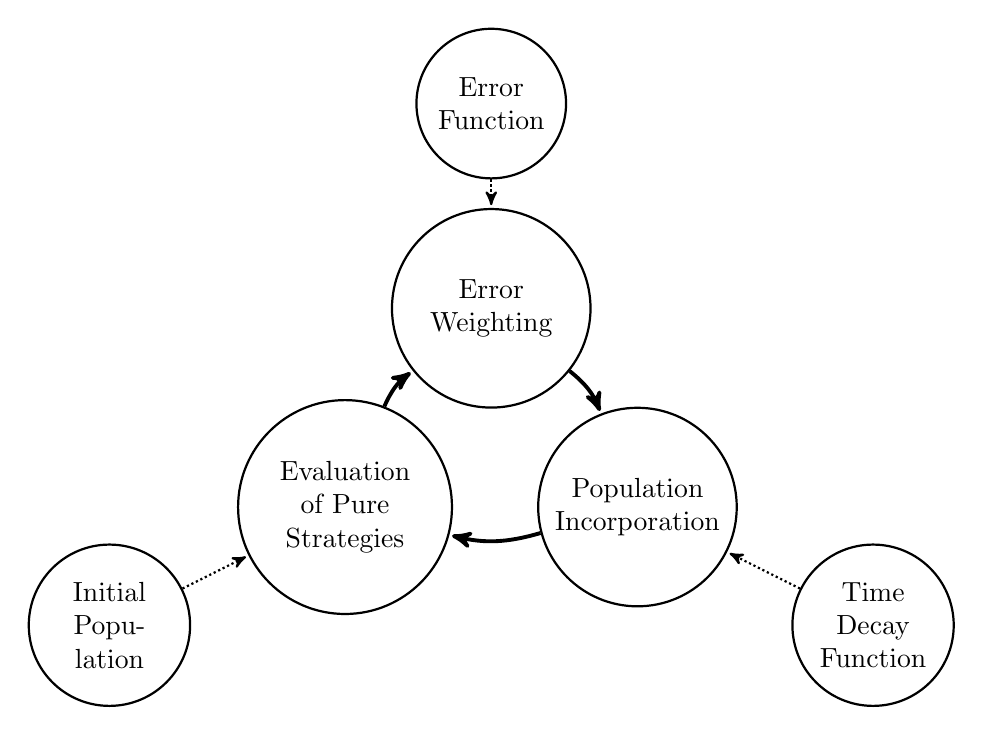
\begin{tikzpicture}[->,>=stealth',shorten >=1pt,auto,node distance=1.7cm,
                    thick,main node/.style={circle,draw}]

\node[main node] (E1) at (0cm, 1.6cm) [align=center, minimum size=1.5cm, text width=2.1cm] {Error\\Weighting};
\node[main node] (P1) at (1.857cm, -0.924cm) [align=center, minimum size=1.5cm, text width=2.1cm] {Population\\Incorporation};
\node[main node] (S1) at (-1.857cm, -0.924cm) [align=center, minimum size=1.5cm, text width=2.1cm] {Evaluation\\of Pure\\Strategies};

\node[main node] (E2) at (0cm, 4.2cm) [align=center, inner sep=2pt, minimum size=1.9cm, text width=1.5cm] {Error\\Function};
\node[main node] (P2) at (4.849cm, -2.425cm) [align=center, inner sep=2pt, minimum size=1.9cm, text width=1.5cm] {Time Decay Function};
\node[main node] (S2) at (-4.849cm, -2.425cm) [align=center, inner sep=2pt, minimum size=1.9cm, text width=1.5cm] {Initial Population};

\path
    (E1) edge [bend left=15,line width=1.4pt] node {} (P1)
    (P1) edge [bend left=15,line width=1.4pt] node {} (S1)
    (S1) edge [bend left=15,line width=1.4pt] node {} (E1)
    (E2) edge [densely dotted] node {} (E1)
    (P2) edge [densely dotted] node {} (P1)
    (S2) edge [densely dotted] node {} (S1)
    ;
\end{tikzpicture}
\end{center}
\caption{diagram of iteration loop}
\end{figure}
The Iteration of the evolutionary process consists of an initial population $P$ and consists of repeating the following 3 steps a finite number of times:

1. The population is used to evaluate the growths of all the pure strategies of the game

2. The strategies are weighted using the error function $r$ on their growths.

3. The weighted average of the strategies steady-state populations are incorporated into the population by factor given by the time delay function $T$.

which is mathematically specified by the by the previous section's boxed equation.

\section{An Example Process}

We give a simple example to illustrate the dynamics of the process with the choice of error and time-decay function.
Let us consider the simple and well-studied classical evolutionary game of Paper-Scissors-Rock.
The game is stateless, consists of 3 pure strategies, and is known for its potential for cyclic instabilities (artificial or otherwise):

\subsection{Paper-Scissors-Rock game}
\begin{center}
\fbox{\begin{minipage}{16cm}
We consider that there is a large population of individuals each of whom are each 'programmed' (in some sense) to play one of 3 different strategies in a symmetric two player game.
The evolutionary process selects random individuals to play the game where the outcome determines reproductive potential of the selected participants.
The game features three strategies called 'Rock'($R$), 'Paper'($P$), and 'Scissors'($S$) and are mutually as good as each other.
$P$ scores a positively higher payoff against $R$ to the same extent that $S$ scores a higher payoff against $P$, and $R$ against $S$.
and vice versa: that $S$ scores a positively lower payoff against $R$ to the same extent that $R$ scores a lower payoff against $P$, and $P$ against $S$.
and each strategy against itself scores the same against itself as any other strategy.
\end{minipage}}
\end{center}

The most basic game can be described by its matrix $M$:

$$ \pi_1=\begin{bmatrix}
    R_1 \\
    P_1 \\
    S_1 \\
\end{bmatrix}
M
\begin{bmatrix}
    R_2 \\
    P_2 \\
    S_2 \\
\end{bmatrix} ~~~~~~~~~~~~~~~~~~~~~~~~~~~~M=\begin{bmatrix}
    0&-1&1\\
    1&0&-1\\
    -1&1&0
\end{bmatrix} $$

Where between two participants, if the opponents mixed strategy is described by vector $[R_2,P_2,S_2]$ with $R_2$ being the likelyhood of playing 'rock' etc.
and where playing mixed strategy $[R_1,P_1,S_1]$ is going to give expected payoff $\pi_1$.

It should be quite obvious that the game's dynamics are cyclic, that in a population of $R$ players that $P$ players dominate, and in a population of $P$ players that $S$ players dominate, and in $S$ players that $R$ players dominate. It is also worth noting that this particular kind of game (with its cycles) has been famously witnessed in the natural world betwen mating strategies (and colours) of the side-blotched lizard (\textit{Uta stansburiana})\cite{lizards1}

The game can be made more general by being parametarised by factors $a$,$b$ as:

$$ \pi_1=\begin{bmatrix}
    R_1 \\
    P_1 \\
    S_1 \\
\end{bmatrix}
M
\begin{bmatrix}
    R_2 \\
    P_2 \\
    S_2 \\
\end{bmatrix} ~~~~~~~~~~~~~~~~~~~~~~~~~~~~M= \begin{bmatrix}
    0&-b&a\\
    a&0&-b\\
    -b&a&0
\end{bmatrix}~~~~~~~~~~~~~~~a>0,b>0 $$

How does the evolutionary dynamics of such a game depend on factors $a$,$b$?

Well it centrally depends on how one defines the evolutionary process - Josef Hofbauer gives 6 different examples.\cite{psr1} The first of which is according to the replicator equation:

\subsection{Replicator Equation of Paper-Scissors Rock}

If we let $x = [x_1,x_2,x_3]^T$ be the vector describing the population, the replicator eqution is given as:

$$\dot{x}_i=x_i((Mx)_i-x\cdot M x)$$

or for a replicator equation that dosnt need to preserve normalisation:

$$\dot{x}_i=x_i(Mx)_i=x_ig_i(x,t)$$

A simple finite differences gives numerical scheme for timestep $dt$:

$$x^{t+1}_i~~\propto ~~x^{t}_i+dt(Mx^{t})_ix^{t}_i~~~~~~~~~~~~~~~~~~~\text{where}~~x^{t+1}~~\text{is normalised every turn}$$

Example images of the time-evolution according to the replicator equation are shown in the following figure:

\begin{figure}[ht]
\centering
\includegraphics[width=0.8\linewidth]{rps1}
\caption{Replicator dynamics for Rock-Paper-Scissors games:
$a>b$ versus $a<b$, credit to Hofbauer\cite{psr1}}
\label{fig:states}
\end{figure}

Notice that the evolution either cycles inwards towards $x=[\frac{1}{3},\frac{1}{3},\frac{1}{3}]^T$ or outwards depending on the relative values of $a$ and $b$ (and also form complete orbits in the case $a=b$ - as shown in the following figure).
The replicator is continuously replacing the population with strategies directly in proportion to their presence multiplied by their payoff.
When $a>b$ then the game dynamics tend to hinge on opponens trying to choose the right strategy in the presence of the others which tends to make things wash-out evenly.
however when $a<b$ that the game dynamics tend to hinge on opponents trying not to choose the wrong strategy in the presence of the others which increases differences and leads to astable cycles.

\begin{figure}[ht]
\centering
\includegraphics[width=0.8\linewidth]{orbit1}
\caption{Replicator dynamic orbits for Rock-Paper-Scissors games: (left) has orbits for $a=b$ and (right) has the same orbit for $a$ slightly greater than $b$ but with two very different timesteps}
\label{fig:states}
\end{figure}

It is also important to note that in some cases where there might otherwise be stability, that descretising the iteration with a finite time-step may introduce astability (as witnessed in the above figure where the otherwise converging orbit is flung outwards due to the time-step over-reach).

\subsection{Best Response Incorporation of Paper-Scissors Rock}

Hofbauer\cite{psr1} also gives visualisations of best-response incorporation as shown in the following figure:

\begin{figure}[ht]
\centering
\includegraphics[width=0.8\linewidth]{rps2}
\caption{Best response dynamics for Rock-Paper-Scissors
games, left one: $a\ge b$, right one: $a < b$, credit to Hofbauer\cite{psr1}}
\label{fig:states}
\end{figure}

the equation for best reply incorporation is:

$$ \dot{x}=BR(x)-x $$

where $BR$ is function that returns the strategy (potentially mixed) that is the 'best reply' to population $x$ (if everyone is playing rock, the best reply is paper etc.)

which is also equivilant to unnormalised form:

$$ \dot{x}_i=BR(x)_i=h_i(x,t) $$

What is interesting is that where in cases of $a<b$ where replicator equation would tend to outward cycling that the Best reply incorporation tends to a much more constrainted cycle.
It is evident that if we model the process of evolution as continuously having all mutations present (as growing and decaying together) as per the replicator equation, then we can get quite different dynamics than if we modeled the process of evolution as reliably introducing a single rare significantly advantageous mutation at a time - as per best reply incorporation.

\subsection{Error function iteration of Paper-Scissors Rock}

a final example from Hofbauer\cite{psr1} is that of 'smoothed best replies':

\begin{figure}[ht]
\centering
\includegraphics[width=0.8\linewidth]{rps3}
\caption{Logit dynamics for Rock-Paper-Scissors games: $a \ge b$
versus $a < b$, credit to Hofbauer\cite{psr1}}
\label{fig:states}
\end{figure}

The 'smoothed best replies' equation used by Hofbauer\cite{psr1} is given as:

$$ \dot{x}=L\left(\frac{Ax}{\epsilon}\right) -x$$

which is also equivilant to unnormalised form:

$$ \dot{x}_i=L\left(\frac{Ax}{\epsilon}\right)=h_i(x,t) $$

where (as also in McNamara et.al\cite{errors1}) $\epsilon$ is the degree of smoothing, Hofbauer particularly chooses $L$ to be the logit function - though he happily acknowledges other choices:

$$ L_k(u) = \frac{e^{u_k}}{\sum_je^{u_j}} $$

Which is quite straightforwardly equivilant to an error function of the form:

$$R(a,b) = e^{\frac{a}{\epsilon}}$$

The general 'smoothed best replies'\cite{psr1} or 'best reply with errors'\cite{errors1} are constructed from a conceptual basis of having perterbations in the best reply function.

There are several things worth noting, the first of which is that smoothed best replies can warp the position of stability points (depending on the strength of the smoothing) and also that the less the smoothing the more vulnerable the convergence of the simulation is to the size of timesteps.

\subsection{Skewed Paper-Scissors-Rock game}

It is possible to skew the stable dynamics of the game towards or away from any of the three strategies.
if we introduce parameters $A$,$B$,$C$ into the game matrix as:

$$ \pi_1=\begin{bmatrix}
    R_1 \\
    P_1 \\
    S_1 \\
\end{bmatrix}
M
\begin{bmatrix}
    R_2 \\
    P_2 \\
    S_2 \\
\end{bmatrix} ~~~~~~~~~~~~~~~~~~~~~~~~~~~~M= \begin{bmatrix}
    0&-Bb&Ca\\
    Aa&0&-Cb\\
    -Ab&Ba&0
\end{bmatrix}~~~~~~~~~~~~~~~a>0,b>0,A>0,B>0,C>0 $$

having $B<A$,$B<C$ would have the game skewed towards the Paper strategy as can be seen in the following figure.
What is also shown is the change in the stable point with the different values of smoothing ($\epsilon$) on the best response incorporation.
That the higher the $\epsilon$ value (ie the greater the smoothing) the more the true equilibrium point is damped out of the response towards the center.

\begin{figure}[ht]
\centering
\includegraphics[width=0.8\linewidth]{orbit2}
\caption{(left) is replicator equation demonstrating skewed convergence for $B=0.3,A=C=1,a=0.5,b=0.4$, (right) is logit smoothed best replies showing stability-point drifting for different $\epsilon$ for $B=0.3,A=C=1,a=0.5,b=0.1$, values of $\epsilon$ are 0,0.01,0.05,0.1,0.15,0.2,0.25 (0 is equal to direct best reply incorporation and is most angular curve; all curves start from the same point)}
\label{fig:states}
\end{figure}

It is also possible to see what happens to best response incorporation (with and without error) in the context of varying timesteps:
The following figure shows the evolution of the system of best responses with and without a large timestep and also with and without errors in the best response.
It is important to note that having even a relatively small error incorporated into the best response brings efficient convergence even to the large timestep.

\begin{figure}[ht]
\centering
\includegraphics[width=0.8\linewidth]{orbit3}
\caption{The responses from an $A=B=C=1$ game with $a=0.5,b=0.1$ of two curves one with timestep 0.001 and the other with 0.2. (left) is the best response incorporation without error for two curves noticing that the one with larger timestep has large 3-step triangular oscillations. (right) is the same graph with a logit error incorporation with $\epsilon=0.05$}
\label{fig:states}
\end{figure}

It is also known that introducing smoothing error into the best reply function is not the only way to increase probability of convergence, but also introducing a slowly-decaying timestep, as the following figure demonstrates.
Having a slowly decaying timestep nessisarily leads to slower convergence on the fine-detail, but is obviously bias-free (unlike error smoothing).

\begin{figure}[ht]
\centering
\includegraphics[width=0.4\linewidth]{orbit4}
\caption{The responses from an $A=B=C=1$ game with $a=0.5,b=0.1$ of two curves one with timestep 0.4 and the other is the same with a harmonically decaying timestep ($ \frac{0.4}{2},\frac{0.4}{3},\frac{0.4}{4},\frac{0.4}{5}\dots $).}
\label{fig:states}
\end{figure}

Hopefully between these examples it can be seen that there is an artfull tradeoff between the expected time-to-convergence, the sizing of the timesteps, the potential for artificial oscillations and the tollerance for bias introduced by error smoothing.
And that this should be the case generally, for simple games such as Paper-Scissors-Rock as well as more complicated games.

\section{Total game specification}

All the elements that need to be specified are:
\begin{itemize}[leftmargin=*,labelsep=4mm]
\item	$S$ is a finite set of states
\item	$A_s$ is finite set of actions available from a state $s\in S$; $A=\cup_s A_s$; $A_s \ne \emptyset$
\item	$T_s(a,P)$ is the transmission to state $s\in S$ when action $a\in A$ is taken in the context of $P$; $T_s\ge 0$\\ where $P(s)$ is the proportion of the population in state $s\in S$; $P(s)\ge 0$; $\sum_{s\in S}P(s)=1$
\item	$R(a,b)$ is a error function
\item	$T(t)$ is timestep function
\item	The set of starting points $P$
\end{itemize}

In order to effectively input such a game into configuration for a computer solver it helps to ennumerate the states $S=\{s_0,s_1,s_2,\dots\}$, and actions $A=\{a_0,a_1,a_2,\dots\}$, and to encode what actions (rows) are available to what states (columns) as ones (denoting availability) and zeros (denoting unavailability) in a matrix which we will call a 'switch-table'.

For instance the following matrix identifies that actions $a_0,a_2,a_3$ are available to state $s_0$; $a_1,a_3$ available to $s_1$ and $a_0,a_2$ available to $s_2$.

$$ \text{Switch Table}= \begin{bmatrix}
    1&0&1 \\
    0&1&0 \\
    1&0&1 \\
    1&1&0
\end{bmatrix} $$

Note that there is nothing in the construction of the game that prohibits the same action from being available to multiple states, only that a given state must have atleast one available action.
Since the states and actions are all enumerated, so too the transmissions as functions of $P$ can be ordered into matrix form.

If we consider that the ordered actions are columns, and resultant transmission to states are rows then we have a matrix encoding all the tranmssions, which we call a 'choice table'.

For instance, the following matrix identifies all the relevant transmission factors, as example:

$$ \text{Choice Table} = \begin{bmatrix}
    T_{s_{0}}(a_0,P)&T_{s_{0}}(a_1,P)&T_{s_{0}}(a_2,P)&T_{s_{0}}(a_3,P) \\
    T_{s_{1}}(a_0,P)&T_{s_{1}}(a_1,P)&T_{s_{1}}(a_2,P)&T_{s_{1}}(a_3,P) \\
    T_{s_{2}}(a_0,P)&T_{s_{2}}(a_1,P)&T_{s_{2}}(a_2,P)&T_{s_{2}}(a_3,P)
\end{bmatrix} = \begin{bmatrix}
    1&P(s_2)^2+0.2&0.8&1-P(s_1)\\
    P(s_0)&P(s_1)P(s_2)&1&0.4P(s_0)\\
    0.3&P(s_0)&1&1-P(s_0)
\end{bmatrix} $$

The above matrix identifies that any action $a_0$ has a transmission of 1 to state $s_0$, and that action $a_1$ has a transmission to state $s_2$ equal to the proportion (between 0 and 1) of individuals in state $s_0$. etc.
In this way, it is possible to define all the states,actions and transmissions by two matricies.
There only remains three additional components: the error function $R(a,b)$, the timstep function $T(t)$ and the initial ponts of $P$.
We note that there may be multiple points of convergence for a given game, and therefore it is reccommened to initialise the game with a set of different starting points $P$.



\section{Objection: what about the mixed strategies?}

Good question!

It is noticed in the specification of the game loop that we only evaluate and incorporate the pure strategies based on their payoff, why should we not consider the possibility that a mixed mutant strategy might perform better than the pure ones and thus define the direction that evolution should take?
As It turns out, the best response strategy is \textit{always} a pure strategy - and this makes it sufficient to discard the potential infinity of mixed strategies in our game iteration.

But to see this we need to make comparrison with Classical Evolutioary game dynamics and to extend the reasoning by further developing the matrix representation of the game as briefly aluded to above.

In classical evolutionary game dynamics, where the payoff is determined by the application of a Matrix to the strategy then the result is trivial because of the linearity of matrix multiplication.
If in a classical game our pure strategies are $a_0,a_1,a_2,\dots$ with payoffs $\pi_0,\pi_1,\pi_2,\dots$ (in the context of the population) then if one of the pure strategies has a greater payoff than the others, say $\pi_0>\pi_1\ge\pi_2\ge\pi_3\dots$ the that strategy has the highest possible payoff.
This is the case simply because any mixed combination of strategies $\beta_0a_0+\beta_1a_1+\beta_2a_2+\dots$ (with $\sum_i\beta_i=1$) has payoff $\beta_0\pi_0+\beta_1\pi_1+\beta_2\pi_2+\dots$ which is less than $\pi_0$ (or ever equal to it when $\beta_0=1,\beta_{i\ne0}=0$) and in this way no mixed strategy can achieve higher payoff than the greatest pure strategy.

However in our case - where we depart from classical evolutionary game dynamics - the same reasoning is simply not valid.
This is primarily the case because, rather than determining our payoffs via application of a linear operator we have a non-linear transformation.
If we have two strategies $z_0$ and $z_1$ the growth associated with playing a mixed combination of them has no nessisary relation to the growth of them individually.
In order to see this we need to develop the matrix representation of the game as described above.

If we take a switch table (the one above), it is important to note that it dosnt encode the probabilities of what actions being taken, only what actions are available to be taken.
However it is very possible to 'weight' the 1 elements of the switch table to encode a specific strategy.
consider switch table:

$$ \text{Switch Table}= \begin{bmatrix}
    1&0&1 \\
    0&1&0 \\
    1&0&1 \\
    1&1&0
\end{bmatrix} $$

state $s_2$ has two actions available to it (as indicated by the two 1s in the second column), these two 1s identify that actions $a_1$ and $a_3$ are available from $s_2$.
A strategy (mixed or pure) would assign the probabilities of the actions taken (which would sum to 1). The same reasoning applies to all the other states.
Thus the space of mixed strategies of the game is described by the following matricies:

$$ \text{Weighted Switch Table}= \begin{bmatrix}
    \delta_{0,0}&0&\delta_{2,0} \\
    0&\delta_{1,0}&0 \\
    \delta_{0,1}&0&\delta_{0,1} \\
    \delta_{0,2}&\delta_{1,1}&0
\end{bmatrix} $$
where $(\delta_{0,0},\delta_{0,1},\delta_{0,2}) \in \Delta_3$, $(\delta_{1,0},\delta_{1,1})\in\Delta_2$, $(\delta_{2,0},\delta_{2,1})\in\Delta_2$ where $\Delta_i$ is the 'unit simplex' (the space where the $i$ positive numbers add to 1):
$$ \Delta_i=\left\{x\in\mathbb{R}^{m_i}_+:\sum_{k=0}^ix_k=1\right\} $$
And the mixed strategy space of the game is thus $\Delta_3\times\Delta_2\times\Delta_2$

A particular example of such a strategy is encoded in the following matrix:

$$ \text{Weighted Switch Table}=S_{witch=} \begin{bmatrix}
    0.4&0&0.5 \\
    0&0.1&0 \\
    0.3&0&0.5 \\
    0.3&0.9&0
\end{bmatrix} $$

Is an example of a matrix which uniquely identifies a strategy of the game, (where in state $s_1$ that actions $a_1$ and $a_3$ would be taken with probabilities respectively of 0.1 and 0.9 etc.)
And if we apply this 'weighted switch table' matrix to a population vector $[p(s_0),p(s_1),p(s_2)]^T$ (where $p(s_0)$ is proportion of the sample population in state $s_0$ etc) we get a vector with the proportions of what actions are taken in the population $[E(a_0),E(a_1),E(a_2),E(a_3)]^T$ (where $E$ is expectation operator).
So for instance: the above matrix identifies a strategy, which if it is applied to a population which is 50\% in $s_0$, 30\% in $s_1$ and 20\% in $s_2$ we get:

$$ \begin{bmatrix}
    0.4&0&0.5 \\
    0&0.1&0 \\
    0.3&0&0.5 \\
    0.3&0.9&0
\end{bmatrix}\begin{bmatrix}
    0.5 \\
    0.3 \\
    0.2
\end{bmatrix} = \begin{bmatrix}
    0.3 \\
    0.03 \\
    0.25 \\
    0.42
\end{bmatrix} $$

So in that population that action $a_0$ will be taken ten times more than $a_1$ etc.
and that vector of action proportions can be converted into expected transmission by application of the 'choice table' matrix:

$$C_{hoice}
\begin{bmatrix}
    0.3 \\
    0.03 \\
    0.25 \\
    0.42
\end{bmatrix}
=
\begin{bmatrix}
    1&P(s_2)^2+0.2&0.8&1-P(s_1)\\
    P(s_0)&P(s_1)P(s_2)&1&0.4P(s_0)\\
    0.3&P(s_0)&1&1-P(s_0)
\end{bmatrix}
\begin{bmatrix}
    0.3 \\
    0.03 \\
    0.25 \\
    0.42
\end{bmatrix} = \begin{bmatrix}
    0.926+0.03P(s_2)^2-0.42P(s_1) \\
    0.25+0.468P(s_0)+0.03P(s_1)(s_2) \\
    0.76-0.39P(s_0)
\end{bmatrix}
$$

And thus he resultant transmission to state $s_2$ will be equal to $0.76-0.39P(s_0)$. ie. that the higher the proportion of individuals in state $s_0$ the lower the local poulation of population $[0.5,0.3,0.2]^T$ playing the strategy described by the weighted switch table will transmit to state $s_2$ etc.

What we have done, is to apply the choice table matrix (identifying the transmissions as influenced by population) to the result of weighted switch table (identifying the strategy) applied to the population vector.
From applying the first matrix we get proportions of actions from occupations of states, and from the second we get transmissions to states from proportions of actions.
This intermediate stage can be eliminated by simply multiplying the matricies together.
$$ M = C_{hoice}S_{witch} $$
Now, $M$ is our 'transmission matrix' (which gives state transmissions from state occupations), who's eigenvalue determines the growth and hence fitness/payoff of the strategy encoded in the weighted switch-table.

\subsection{Non-Linearity}

if we have two strategies $z_1$ and $z_2$ who have corresponding weighted swtich-table matricies $S_1$ and $S_2$ and the population has choice matrix $C$, then the strategies themselves have growth rates $\lambda_1$ and $\lambda_2$ for:
$$\lambda_1V_1=CS_1V_1$$
$$\lambda_2V_2=CS_2V_2$$
however the growth-rate $\lambda_3$ of a mixed strategy of the two (as for instance 50:50) has no guaranteed relation to either $\lambda_1$ or $\lambda_2$
$$\lambda_3V_3=C(0.5S_1+0.5S_2)V_3$$
$\lambda_3$ could be higher, lower or inbetween $\lambda_1$ and $\lambda_2$

\subsection{Column-wise monotonicity}

consider the difference between the following two strategy $z_1$,$z_2$ switch-tables:

$$ \begin{bmatrix}
    0.4&0&0.5 \\
    0&0.1&0 \\
    0.3&0&0.5 \\
    0.3&0.9&0
\end{bmatrix}~~~~~~~~~~~~~~~~~\begin{bmatrix}
    0.4&0&0.5 \\
    0&0.8&0 \\
    0.3&0&0.5 \\
    0.3&0.2&0
\end{bmatrix}$$

The only difference between them is in the middle column, where the probability of initiating action $a_1$ as opposed to $a_3$ has been shifted.
What we notice is that the growthrate and payoff of each of these strategies $\lambda_1$ and $\lambda_2$ defines the bounds of the growthrate and payoff of any mix of the two strategies.
If $\lambda_1$>$\lambda_2$ (without loss of generality) then if $z_3=\alpha z_1+(1-\alpha) z_2$ for ($0<\alpha<1$) then the growthrate of $z_3$ is $\lambda_3$ and $\lambda_1\ge\lambda_3\ge\lambda_2$.
This is true for all strategies of a single column of a switch-table matrix.
(NOTE: this has been demonstrated to hold by computational enumeration of thousands of real positive matricies - but a mathematical proof is forthcomming)

In this way it is possible to see that between any two strategies that differ in a single column of the switch table, that changing the mixing parameter $\alpha$ will result in a monotonic non-decrease (or non-increase) in growth-rate, hence the greatest (and lowest) growth-rate will occur at extreme $\alpha=0$ or $\alpha=1$.
Between the multiplicity of strategies which define all the strategies that differe in a single column it can be thenceforth seen that the greatest (and lowest) growth-rate will occur at the extreme - where the column consists of a singular 1 and all else 0.
And this reasoning applies to all columns.

Thus the greatest (and lowest) growth-rate occurs for the pure strategies of the game.
And it is by simple ennumeration of the finite pure strategies that it is possible to find the strategy of greatest growth-rate (which is of primary relevance).

\section{A return to Hawk-Dove example}

The Hawk-Dove game outlined before is simple enough to yield analytic soltuion, the derivation of which is given in Appendix A.

In a game is: $$ (C+1)^2+4(DC-D)>0? ~~~~~~\text{and}~~~~~~ \sqrt{(C+1)^2+4(DC-D)} > 2(1-A)(DC-D)+C+1? $$
\begin{itemize}[leftmargin=*,labelsep=3mm]
\item	if so then the Game equilibrium is Hawk-Saturated:$$p=\frac{-(C+1)+\sqrt{(C+1)^2+4(DC-C)}}{2(DC-C)}$$and proportion of Young is$$\frac{\sqrt{DpC(1+p+A)}}{\sqrt{DpC(1+p+A)}+1-pC+DpC}$$
\item	if not then a Hawk-Dove equilibrium exists:$$p=1-A$$and proportion of Young is$$\frac{\sqrt{2A}}{\sqrt{2A}+\sqrt{C(1-A)(D-1)+1}}$$
\end{itemize}

The game itself is sufficiently simple enough to redily conduct simple stochastic simulations to witness the dynamics.
The Moran process is a very simple stochastic model of the evolution of finite populations, where each 'turn' a random individual is chosen for reproduction proportional to its fitness, and a corresponding random individual is chosen for death.
The Moran process is known to yield replicator equation dynamics in the limit of large-populations under specific conditions\cite{stochastic1} and is generally regarded as a cornerstone technique of stochastic evolutionary game dynamics.

We design a simple stochastic simulator ('moran simulator') bassed on the moran process, and who's source-code is shown in Appendix B.
Since our Hawk-Dove game does not feature fitness values \textit{per sei} but ony the expectation of transmission between states, the functions slightly differently from the essential Moran process - though the essential idea remains unchanged.

The simulation selects individuals of a finite population randomly, generates new individuals bassed apon expected transmission and incorporates them into the population by replacing other individuals randomly.
The source code is very simple, easily understood and intuitively yields evolutionary dynamics.

The results of the simulation against analytic prediction are shown in the following figure; in it are shown the value $p$ (the proportion of adults that are agressive at equilibrium) and the proportion of young in the equilibrium population ($\%Y$) against the parameter $A$ for a game of fixed $C$ and $D$.

The Hawk-Dove game is also immediately susceptible to our iterative solver (as described in previous sections), and the results of our solver are juxtaposed against the analytical results and Moran simulator results for the same game in the following figure.

The results strongly show that our iterative solver accurately predicts the evolutionary dynamics in the case of our Hawk-Dove game:

\begin{figure}[H]
\begin{center}
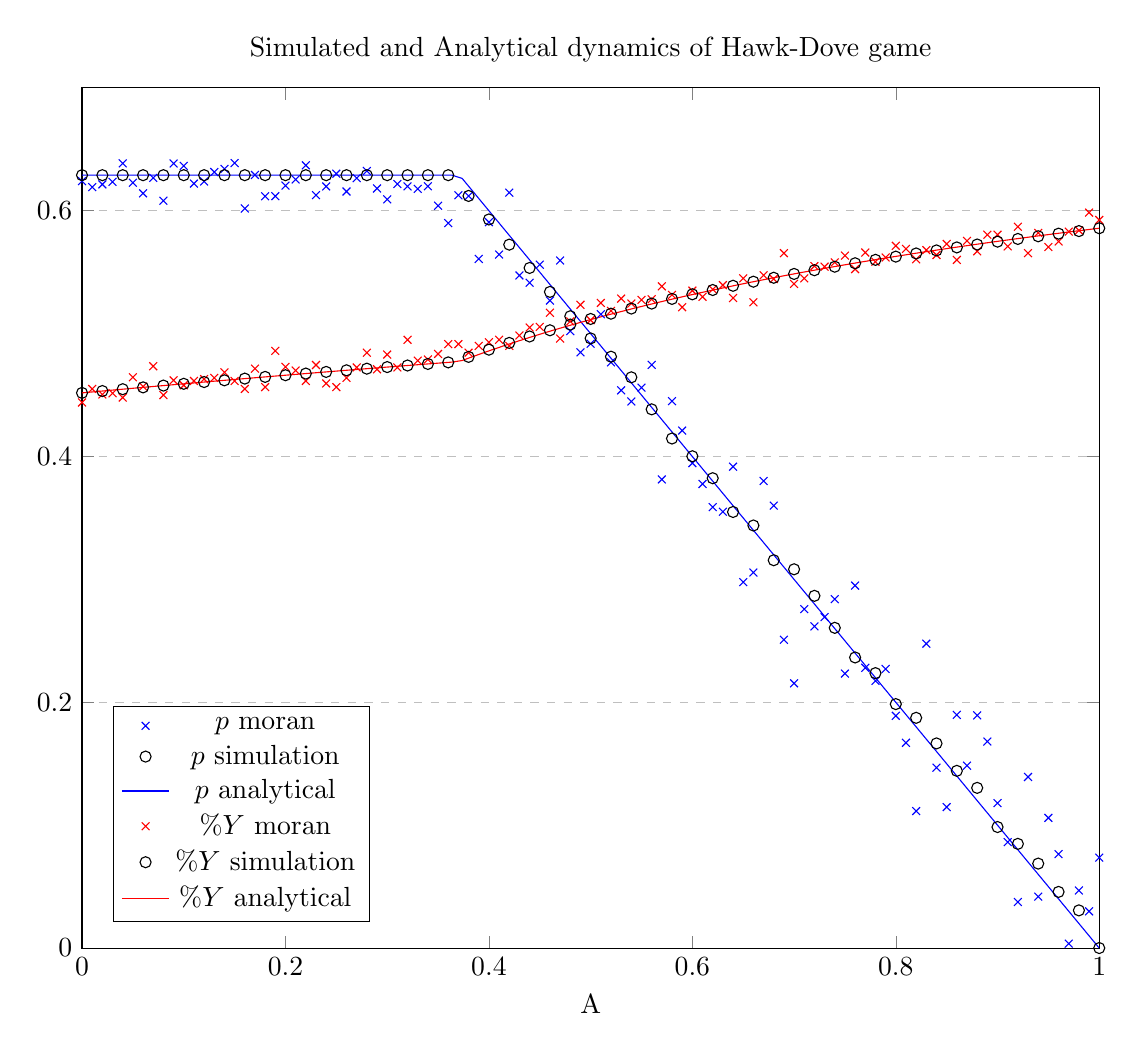
\begin{tikzpicture}
\begin{axis}[
    title={Simulated and Analytical dynamics of Hawk-Dove game},
    xlabel={A},
    xmin=0, xmax=1,
    ymin=0, ymax=0.7,
    xtick={0,0.2,0.4,0.6,0.8,1.0},
    ytick={0,0.2,0.4,0.6,0.8,1.0},
    legend pos=south west,
    ymajorgrids=true,
    grid style=dashed,
]
 
\addplot[
    color=blue,
    mark=x,
only marks,
    ]
    coordinates {
    (0.0,0.6241007194244604)(0.01,0.6192660550458715)(0.02,0.62147406733394)(0.03,0.6235186873290793)(0.04,0.6385869565217391)(0.05,0.6227824463118581)(0.06,0.6141804788213628)(0.07,0.6267806267806267)(0.08,0.6081818181818182)(0.09,0.6384758364312267)(0.1,0.6365313653136532)(0.11,0.6220984215413184)(0.12,0.6238361266294227)(0.13,0.6315298507462687)(0.14,0.6340545625587959)(0.15,0.6388115134633241)(0.16,0.6018348623853211)(0.17,0.6291390728476821)(0.18,0.6117755289788408)(0.19,0.6118677042801557)(0.2,0.6204933586337761)(0.21,0.6254716981132076)(0.22,0.6369545032497679)(0.23,0.6127497621313035)(0.24,0.6197964847363552)(0.25,0.6301747930082797)(0.26,0.6156716417910447)(0.27,0.6265402843601896)(0.28,0.6323957322987391)(0.29,0.6181474480151229)(0.3,0.6092843326885881)(0.31,0.6218009478672986)(0.32,0.6198019801980198)(0.33,0.617816091954023)(0.34,0.6199616122840691)(0.35000000000000003,0.6040658276863504)(0.36,0.5899705014749262)(0.37,0.6125860373647984)(0.38,0.612027158098933)(0.39,0.5607843137254902)(0.4,0.5907297830374754)(0.41000000000000003,0.5643564356435643)(0.42,0.6147058823529412)(0.43,0.5473579262213359)(0.44,0.5414141414141415)(0.45,0.5561172901921132)(0.46,0.5269151138716356)(0.47000000000000003,0.5595238095238095)(0.48,0.5020408163265306)(0.49,0.48478488982161594)(0.5,0.4918200408997955)(0.51,0.5157894736842106)(0.52,0.4766355140186916)(0.53,0.45387062566277836)(0.54,0.444794952681388)(0.55,0.4560846560846561)(0.56,0.4745762711864407)(0.5700000000000001,0.38136511375947996)(0.58,0.4450373532550694)(0.59,0.4211076280041797)(0.6,0.3946236559139785)(0.61,0.3776595744680851)(0.62,0.3588362068965517)(0.63,0.3550488599348534)(0.64,0.39171974522292996)(0.65,0.2978021978021978)(0.66,0.3055848261327713)(0.67,0.38011049723756907)(0.68,0.3600439077936334)(0.6900000000000001,0.2508630609896433)(0.7000000000000001,0.21545157780195864)(0.71,0.27582417582417584)(0.72,0.26179775280898876)(0.73,0.26936026936026936)(0.74,0.2839366515837104)(0.75,0.22336769759450173)(0.76,0.29497206703910617)(0.77,0.22811059907834103)(0.78,0.217440543601359)(0.79,0.2271689497716895)(0.8,0.18903150525087514)(0.81,0.16705336426914152)(0.8200000000000001,0.11149032992036405)(0.8300000000000001,0.24768518518518517)(0.84,0.14678899082568808)(0.85,0.11475409836065574)(0.86,0.18977272727272726)(0.87,0.14840989399293286)(0.88,0.18937644341801385)(0.89,0.16805721096543505)(0.9,0.11799761620977355)(0.91,0.08624708624708624)(0.92,0.03753026634382567)(0.93,0.13924050632911392)(0.9400000000000001,0.041866028708133975)(0.9500000000000001,0.10593713620488941)(0.96,0.07647058823529412)(0.97,0.0035971223021582736)(0.98,0.046875)(0.99,0.029887920298879204)(1.0,0.0736196319018405)
    };
\addlegendentry{$p$ moran}
\addplot[
    color=black,
    mark=o,
only marks,
    ]
    coordinates {
    (0,0.6289575409)(0.02,0.6289575408)(0.04,0.6289575408)(0.06,0.6289575408)(0.08,0.6289575408)(0.1,0.6289575407)(0.12,0.6289575407)(0.14,0.6289575407)(0.16,0.6289575406)(0.18,0.6289575406)(0.2,0.6289575406)(0.22,0.6289575406)(0.24,0.6289575405)(0.26,0.6289575405)(0.28,0.6289575405)(0.3,0.6289575405)(0.32,0.6289575404)(0.34,0.6289575404)(0.36,0.6289575404)(0.38,0.612076522)(0.4,0.5929204369)(0.42,0.5724290654)(0.44,0.5534669904)(0.46,0.5339752456)(0.48,0.514153272)(0.5,0.4961318585)(0.52,0.4812381284)(0.54,0.4644582026)(0.56,0.4384020896)(0.58,0.4146634204)(0.6,0.4002183477)(0.62,0.3823539664)(0.64,0.3548949283)(0.66,0.3438717262)(0.68,0.3156223198)(0.7,0.3082387843)(0.72,0.2866354793)(0.74,0.2605980834)(0.76,0.2364928021)(0.78,0.2237394815)(0.8,0.198538722)(0.82,0.1873662614)(0.84,0.1665438528)(0.86,0.1442164537)(0.88,0.130370258)(0.9,0.0985018176)(0.92,0.0848022188)(0.94,0.0687530764)(0.96,0.0457160899)(0.98,0.0306759601)(1,0.000026934)
    };
\addlegendentry{$p$ simulation}
\addplot [
    domain=0:1, 
    samples=100, 
    color=blue,
    ]
    {min(1-x,(-1*(0.7+1)+sqrt((0.7+1)^2+4*(0.75*0.7-0.7)))/(2*(0.75*0.7-0.7)))};
\addlegendentry{$p$ analytical}

\addplot[
    color=red,
    mark=x,
only marks,
    ]
    coordinates {
    (0.0,0.444)(0.01,0.455)(0.02,0.4505)(0.03,0.4515)(0.04,0.448)(0.05,0.4645)(0.06,0.457)(0.07,0.4735)(0.08,0.45)(0.09,0.462)(0.1,0.458)(0.11,0.4615)(0.12,0.463)(0.13,0.464)(0.14,0.4685)(0.15,0.4615)(0.16,0.455)(0.17,0.4715)(0.18,0.4565)(0.19,0.486)(0.2,0.473)(0.21,0.47)(0.22,0.4615)(0.23,0.4745)(0.24,0.4595)(0.25,0.4565)(0.26,0.464)(0.27,0.4725)(0.28,0.4845)(0.29,0.471)(0.3,0.483)(0.31,0.4725)(0.32,0.495)(0.33,0.478)(0.34,0.479)(0.35000000000000003,0.4835)(0.36,0.4915)(0.37,0.4915)(0.38,0.4845)(0.39,0.49)(0.4,0.493)(0.41000000000000003,0.495)(0.42,0.49)(0.43,0.4985)(0.44,0.505)(0.45,0.5055)(0.46,0.517)(0.47000000000000003,0.496)(0.48,0.51)(0.49,0.5235)(0.5,0.511)(0.51,0.525)(0.52,0.5185)(0.53,0.5285)(0.54,0.5245)(0.55,0.5275)(0.56,0.528)(0.5700000000000001,0.5385)(0.58,0.5315)(0.59,0.5215)(0.6,0.535)(0.61,0.53)(0.62,0.536)(0.63,0.5395)(0.64,0.529)(0.65,0.545)(0.66,0.5255)(0.67,0.5475)(0.68,0.5445)(0.6900000000000001,0.5655)(0.7000000000000001,0.5405)(0.71,0.545)(0.72,0.555)(0.73,0.5545)(0.74,0.558)(0.75,0.5635)(0.76,0.5525)(0.77,0.566)(0.78,0.5585)(0.79,0.562)(0.8,0.5715)(0.81,0.569)(0.8200000000000001,0.5605)(0.8300000000000001,0.568)(0.84,0.564)(0.85,0.573)(0.86,0.56)(0.87,0.5755)(0.88,0.567)(0.89,0.5805)(0.9,0.5805)(0.91,0.571)(0.92,0.587)(0.93,0.5655)(0.9400000000000001,0.582)(0.9500000000000001,0.5705)(0.96,0.575)(0.97,0.583)(0.98,0.584)(0.99,0.5985)(1.0,0.5925)
    };
\addlegendentry{$\%Y$ moran}

\addplot[
    color=black,
    mark=o,
only marks,
    ]
    coordinates {
    (0,0.4517879923)(0.02,0.4532995325)(0.04,0.454793696)(0.06,0.4562708607)(0.08,0.4577313924)(0.1,0.4591756452)(0.12,0.4606039617)(0.14,0.4620166739)(0.16,0.4634141037)(0.18,0.4647965628)(0.2,0.4661643536)(0.22,0.4675177693)(0.24,0.4688570945)(0.26,0.4701826053)(0.28,0.4714945698)(0.3,0.4727932483)(0.32,0.4740788938)(0.34,0.4753517521)(0.36,0.4766120619)(0.38,0.481090244)(0.4,0.4869661083)(0.42,0.4924735851)(0.44,0.4976896808)(0.46,0.5027316219)(0.48,0.5073749581)(0.5,0.5119454382)(0.52,0.5162481778)(0.54,0.5204110004)(0.56,0.5244511101)(0.58,0.5282664683)(0.6,0.5320149674)(0.62,0.5355073402)(0.64,0.5389475511)(0.66,0.5422738195)(0.68,0.5454718357)(0.7,0.5485898114)(0.72,0.5516044024)(0.74,0.5544683829)(0.76,0.5572789613)(0.78,0.5600580262)(0.8,0.5626724267)(0.82,0.5652437768)(0.84,0.5677256814)(0.86,0.5701638369)(0.88,0.5725295204)(0.9,0.5748670415)(0.92,0.5770550208)(0.94,0.5792379959)(0.96,0.5813724357)(0.98,0.5834521911)(1,0.5857672831)
    };
\addlegendentry{$\%Y$ simulation}

\addplot [
    domain=0:1, 
    samples=100, 
    color=red,
    ]
    {max(sqrt(2*x)/(sqrt(2*x)+sqrt(0.7*(1-x)*(0.75-1)+1)), (sqrt(0.75*0.6289575465860742*0.7*(1+0.6289575465860742+x)))/(sqrt(0.75*0.6289575465860742*0.7*(1+0.6289575465860742+x))+1-0.6289575465860742*0.7+0.75*0.6289575465860742*0.7))};
\addlegendentry{$\%Y$ analytical}
 
\end{axis}
\end{tikzpicture}
\caption{Dynamics of the Hawk-Dove game across parameter $A$, with $D = 0.75$ and $C = 0.70$\\ shown are results for $p$ as well as proportion Young $\%Y$ for Moran stochastic simulation, analytical prediction, and our software solver's results}
\end{center}
\end{figure}

The Hawk-Dove game described in this paper with the results above was a simplification of Eitan Altman's mulit-state Hawk-Dove MDEG game\cite{markov5}. We failed to impliment his game exactly, because his game assigned negative fitness values (which simply could not easily be interpreted terms of number of offspring...)
We also failed to witness the dynamics he claimed would be apparent.

\section{A Bigger example - And this one has Teeth!}

Some of the claims surrounding Evolutionary Psychology are felt to be controversial - not only just its results and findings, but also as a venture itself.
Seeking and solidifying theories surrounding the Evolution of behaviors (particularly in humans) is claimed to be generally incongruent with ideas purportedly present in the social sciences and at-large.

Some purport the ideological target of the attack is the supposed 'standard social science model (SSSM)' \cite{adaptedmind} about which it is alleged "Most contemporary sociologists will find the basic elements ofthe SSSM to be both familiar and unobjectionable" \cite{darwinrevolution} and are identified as being in discord with the basic tennents of evolutionary explanation as applied to the human mind\cite{evolutionhandbook}.
The primary issue is the famous 'nature-vs-nurture' debate, and particularly discordant ideas include the 'blank-slate' hypothesis (also known as \textit{tabula rasa} - that all (or most) knowledge (and/or behavior dispositions) comes from experience and perception) and 'cultural-determinism' (that culture and environment are major and primary influences on a person's behavior and identity).
Some authors go so far as to directly enumerate and individually address objections and ideological concerns surrounding and implications of the venture "Why are so many social-cultural anthropologists so scornful of evolutionary psychology and sociobiology? Whence comes this impulse to stick one’s finger in the Darwinian eye whenever it dares to gaze at human behavior?" \cite{missingrevolution}

Yet the developing of evolutionary explanations for human behavior is purported to be a relatively successfull endeavour by proponents. Proponents claim wide-reaching ideological and social implications "evolutionary psychology is a field of research that has revolutionized how we understand human psychological mechanisms and how they interact with social, cultural, and ecological variables to produce manifest behavior"\cite{feminism}
And armed with a collected array of sociological experiments have published a variety of evolutionary hypotheses as explanations.\cite{socialisation}

Yet there seems to be a distinct step between recognising sociological results (no matter how universal) and justifiably (or not) embracing an evolutionary explanation of the results.
And a central part of the proces consists of assessing the plausibility of the evolutionary explanation in itself, rather than embracing a particular evolutionary explanation as a tenuous 'just-so' story \cite{justso}

Although there is documented several avenues of investigating and supporting evolutionary claims \cite{confirmation} one of the avenues that seems moderately explored is the developing of computational models/simulations to help confirm or disconfirm proposed hypotheses.  As an example instance in \cite{altruism} and \cite{altruism2} there is developed a computational models for the hypothesis of the emergence of Altruism via sexual selection.
The relatively weak epistemic principle would be simply, that if a sufficiently simple and non-question-begging model (computational or otherwise) of a proposed evolutionary hypothesis could not be developed, then it might be seen to count against the hypothesis.

We present a simple computational model to examine the hypothetical evolutionary relationship between paternal uncertainty (that a father cannot redily know if the child is his genetic offspring) and paternal non-investment in the child-rearing - a hypothesis about which has had some dispute \cite{paternity1}\cite{paternity2} and to our knowledge has never been mathematically or computationally modelled.

\subsection{The Elements}

In order to model an answer to the question:
\begin{center}
\fbox{\begin{minipage}{10cm}
"What is the general evolutionary relationship \\$~~~~~~~~~~~~~~~~~~~~~$between paternal uncertainty and paternal investment?" 
\end{minipage}}
\end{center}

We need to define the elements and behaviors between the elements that belong to the model.
By doing this we will nessisarily exclude some factors (which may or may not turn out to be important), however generally the more minimal and simplistic our model the more robust it would seem in its potential to correspond to the real world - if for no other reason than for Ockham's razor.

1. The very question itself specifically involves sex: male and female - which for simple modelling will be taken to be binary.

2. It also involves investment of the parents in the offspring as potentially different between the sexes of the adults - Actual-world parental investment is obviously multifaceted, but for simplicity of the model we will model it as being of one of two binary kinds which we will call (for brevity) 'investing' and 'non-investing' available to both sexes (although we could extend this to any finite number of kinds any which way).

By these two binarisations alone we can see that there are 4 possible heterosexual pairing (as directly producing children) combinations in terms of investment: 
\begin{itemize}
  \item Investing Male \& Investing Female
  \item Non-Investing Male \& Investing Female
  \item Investing Male \& Non-Investing Female
  \item Non-Investing Male \& Non-Investing Female
\end{itemize}
And that each of these pairings could lead to different expectation of offspring for the parents. For simplicity we will dictate that there is sex symmetry of investment - that a parent will have same expectation of offspring irrespective of sex. This reduces the possible cases (in terms of number of offspring) to three:
\begin{itemize}
  \item Two Investing Parents
  \item One Investing Parent
  \item No Investing Parents
\end{itemize}
Each of these cases will have expected offspring, which will be left as parameters of the game - as seen later.

4. The question of paternal uncertainty nessisarily connotates the possibility of that one or the other partner may not be faithful. and there is no \textit{a priori} reason to exclude it as a consideration for either sex, so faithfullness will be modeled as a simple binary for both sexes.

By these three binarisations together we can see that there is 8 different kinds of parents and 16 different possible heterosexual combinations.
As a notational shorthand we let "$M_{CI}$" denote an (C)heating \& (I)nvesting (M)ale, and "$F_{FN}$" denote a (F)aithful \& (N)on-investing (F)emale. etc.

Thus the 8 different kinds of adults are: $ M_{FI}, M_{FN}, M_{CI}, M_{CN}, F_{FI}, F_{FN}, F_{CI}, F_{CN} $
And 16 different possible heterosexual pairing combinations:

\begin{table}[h]
    \centering
    \begin{tabular}{ccccc}
        & $F_{FI}$ & $F_{FN}$ & $F_{CI}$ & $F_{CN}$ \\
        \cline{2-5}
        \multicolumn{1}{c|}{$M_{FI}$} & \multicolumn{1}{c|}{$M_{FI}~F_{FI}$} & \multicolumn{1}{c|}{$M_{FI}~F_{FN}$} & \multicolumn{1}{c|}{$M_{FI}~F_{CI}$} & \multicolumn{1}{c|}{$M_{FI}~F_{CN}$} \\
        \cline{2-5}
        \multicolumn{1}{c|}{$M_{FN}$} & \multicolumn{1}{c|}{$M_{FN}~F_{FI}$} & \multicolumn{1}{c|}{$M_{FN}~F_{FN}$} & \multicolumn{1}{c|}{$M_{FN}~F_{CI}$} & \multicolumn{1}{c|}{$M_{FN}~F_{CN}$} \\
        \cline{2-5}
        \multicolumn{1}{c|}{$M_{CI}$} & \multicolumn{1}{c|}{$M_{CI}~F_{FI}$} & \multicolumn{1}{c|}{$M_{CI}~F_{FN}$} & \multicolumn{1}{c|}{$M_{CI}~F_{CI}$} & \multicolumn{1}{c|}{$M_{CI}~F_{CN}$} \\
        \cline{2-5}
        \multicolumn{1}{c|}{$M_{CN}$} & \multicolumn{1}{c|}{$M_{CN}~F_{FI}$} & \multicolumn{1}{c|}{$M_{CN}~F_{FN}$} & \multicolumn{1}{c|}{$M_{CN}~F_{CI}$} & \multicolumn{1}{c|}{$M_{CN}~F_{CN}$} \\
        \cline{2-5}
    \end{tabular}
\end{table}

Each of these pairings may hold different genetic outcomes for each parent. For instance - a faithfull partner matched with a unfaithfull partner might well only have one genetic offspring whereas the other may have two genetic offspring by the same pairing.

4. We stipulate that the pairings occur randomly in a population and that the only thing influencing the number of offspring is the type of the pairing. 

5. We consider all offspring identical - and we introduce a singular (though unnessisary) Baby state ($B$) for computational simplicity

6. We consider that sex is assigned to babies on a 50:50 basis, and that the genetics dictate what type of adult the baby will become if assigned Male and what kind of adult to become if assigned female. Thus there are 16 different 'pure' strategies in the game (as per the table above)

By these constrictions we are explicitly excluding from analysis a host of phenomena such as mate-screening, family and social structures (or perhaps atleast other than a very basic nuclear family structure), non-heterosexual pairings, sex-ratios, age, social status, wealth, environment, health etc. All these considerations may have relevance and their incorporation into a more expansive model may yield further interesting dynamics; We obviously welcome \textit{any} contribution along these lines! - although we try to keep it simple here.

We keep it as simple as possible to embody the basic characteristics sufficient to minimally test the hypothesis (between paternal uncertainty and investment) without introducing superfluous elements.

\subsection{States and Actions}

The States and the flow of individuals between them can be visualised as per the following diagram:

\begin{figure}[H]
\begin{center}
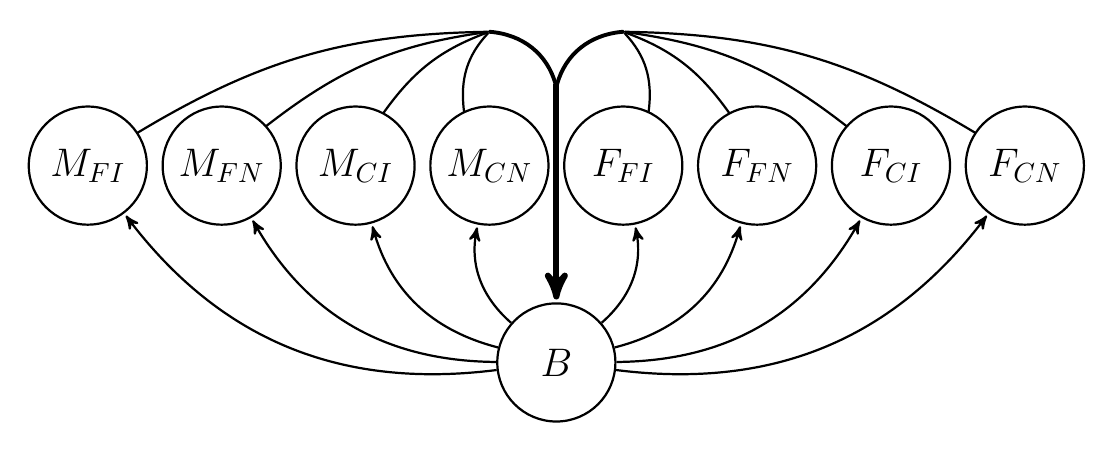
\begin{tikzpicture}[->,>=stealth',shorten >=1pt,auto,node distance=1.7cm,
                    thick,main node/.style={circle,draw,font=\sffamily\Large\bfseries}]

\node[main node] (mfi) [minimum size=1.5cm ]{$M_{FI}$};
\node[main node] (mfn) [minimum size=1.5cm, right of=mfi] {$M_{FN}$};
\node[main node] (mci) [minimum size=1.5cm, right of=mfn] {$M_{CI}$};
\node[main node] (mcn) [minimum size=1.5cm, right of=mci] {$M_{CN}$};
\node[main node] (ffi) [minimum size=1.5cm, right of=mcn] {$F_{FI}$};
\node[main node] (ffn) [minimum size=1.5cm, right of=ffi] {$F_{FN}$};
\node[main node] (fci) [minimum size=1.5cm, right of=ffn] {$F_{CI}$};
\node[main node] (fcn) [minimum size=1.5cm, right of=fci] {$F_{CN}$};
\node[main node] (B) at (5.95cm,-2.5cm) [minimum size=1.5cm] {$B$};

\coordinate[above of=mcn] (a1);
\coordinate[above of=ffi] (a2);
\coordinate (a3) at (5.95cm, 1cm);

  \path[every node/.style={font=\sffamily\small}]
    (B) edge [bend left] node {} (mfi)
        edge [bend left] node {} (mfn)
        edge [bend left] node {} (mci)
        edge [bend left] node {} (mcn)
        edge [bend right] node {} (ffi)
        edge [bend right] node {} (ffn)
        edge [bend right] node {} (fci)
        edge [bend right] node {} (fcn)
    (mfi) edge [bend left=15, -,line cap=rect] node {} (a1)
    (mfn) edge [bend left=15, -,line cap=rect] node {} (a1)
    (mci) edge [bend left=17, -,line cap=rect] node {} (a1)
    (mcn) edge [bend left=25, -,line cap=rect] node {} (a1)
    (ffi) edge [bend right=25, -,line cap=rect] node {} (a2)
    (ffn) edge [bend right=17, -,line cap=rect] node {} (a2)
    (fci) edge [bend right=15, -,line cap=rect] node {} (a2)
    (fcn) edge [bend right=15, -,line cap=rect] node {} (a2)
    (a1) edge [bend left=35, -,line cap=round,line width=1.4pt] node {} (a3)
    (a2) edge [bend right=35, -,line cap=round,line width=1.4pt] node {} (a3)
    (a3) edge [line cap=rect,line width=2.2pt] node {} (B)
;
\end{tikzpicture}
\end{center}
\caption{A diagram showing the flow of individuals between states in the game}
\end{figure}

The set of states are: $$S = \{B, M_{FI}, M_{FN}, M_{CI}, M_{CN}, F_{FI}, F_{FN}, F_{CI}, F_{CN}\}$$
The set of actions available are: $$A = \bigcup_{s \in S} A_s$$
Where the actions available to the baby state are to become a type of Male if assigned Male and a type of Female if assigned Female.
$$A_B = \{a_{M_{\alpha\beta}F_{\gamma\delta}} ~~|~~ \alpha,\gamma\in\{{F,C}\}~~\beta,\delta\in\{{I,N}\}\} = \{a_{M_{FI}F_{FI}}, a_{M_{FI}F_{FN}}, \dots, a_{M_{CN}F_{CN}}\}$$
And each of thoes actions have perfect and total 50:50 transmissions to the respective types of adults:
$$T_{B}(a_{M_{\alpha\beta}F_{\gamma\delta}}, P)=0,~~~~~~~~~ T_{X_{\epsilon\zeta}}(a_{M_{\alpha\beta}F_{\gamma\delta}}, P) = 0.5~~\text{if}~~X_{\epsilon\zeta}=M_{\alpha\beta}~~\text{or}~~X_{\epsilon\zeta}=F_{\gamma\delta}~~\text{else}~~0 $$
ie.$~~ T_{M_{FI}}(a_{M_{FI}F_{CI}}, P) = 0.5,~~ T_{M_{FN}}(a_{M_{FI}F_{CI}}, P) = 0,~~ T_{F_{FN}}(a_{M_{FI}F_{CI}}, P) = 0,~~ T_{F_{CI}}(a_{M_{FI}F_{CI}}, P) = 0.5,~~$etc.\\

Each Adult state has exactly one action each - to participate in pairings and reproduce:
$$A_{X_{\epsilon\zeta}} = \{ r_{X_{\epsilon\zeta}} \}$$

We define that the transmission resulting from such actions be linear with proportions of Adults of the opposite sex.

$$T_{B}(r_{M_{\epsilon\zeta}},P) = \frac{k_{M_{\epsilon\zeta}F_{FI}} P(F_{FI}) + k_{M_{\epsilon\zeta}F_{FN}} P(F_{FN}) + k_{M_{\epsilon\zeta}F_{CI}} P(F_{CI}) + k_{M_{\epsilon\zeta}F_{CN}} P(F_{CN})}{1-P(B)}$$
$$T_{B}(r_{F_{\epsilon\zeta}},P) = \frac{k_{F_{\epsilon\zeta}M_{FI}} P(M_{FI}) + k_{F_{\epsilon\zeta}M_{FN}} P(M_{FN}) + k_{F_{\epsilon\zeta}M_{CI}} P(M_{CI}) + k_{F_{\epsilon\zeta}M_{CN}} P(M_{CN})}{1-P(B)}$$
$$T_{Y_{\alpha\beta}}(X_{\epsilon\zeta},P)=0$$

This linearity coincides with notion that the parings occur randomly in population, and that the pairings are the only determinants of offspring.\footnote{The $1-P(B)$ denominator conducts the scaling so to make all the proportions eg. $P(F_{FI})$ etc. only as amoung the adults}
We note at this point that with the exception of the specification of the factors $k_{X_{\alpha\beta}Y_{\gamma\delta}}$ the game is totally defined and is completely symmetric between sexes.
The remaining task is to specify the 32 $k_{X_{\alpha\beta}Y_{\gamma\delta}}$ factors.
It is also worth mentioning that the only state that has multiple actions available to it is the Baby state (with a total of 16 'pure' strategies) making the mixed strategy space of the game 16 dimensional.

\subsection{The Interaction Factors - $k_{X_{\alpha\beta}Y_{\gamma\delta}}$}

It is quite sufficient and possible to have the 32 $k$ factors as simple parameters of the game, but we will attempt constructions to minimise the factors of the game further - so that we can run simulations across them in order to extract meaningfull results.

\subsubsection{the most minimal case}

Consider that if all Adults participated in exactly one pairing and had two genetic children from the pairing irrespective of investment or faithfullness of themself or partner, that the $k$ factors would all be equal to 2.

\subsubsection{introducing the relevance of investment}

In order to make room for the possibility that parental investment could influence the proportion of thoes children surviving we (as mentioned before) define the three cases $X_0$,$X_1$,$X_2$ of investment:
\begin{itemize}
  \item We denote $X_2$ as child with two Invested Parents - with effective survival probability as $S_2$
  \item We denote $X_1$ as child with one Invested Parent - with effective survival probability as $S_1$
  \item We denote $X_0$ as child with no Invested Parents - with effective survival probability as $S_0$
\end{itemize}

If the only consideration in the simulation was the level of investment then the $k$ factors could be:
$$ k_{X_{\alpha\beta}Y_{\gamma\delta}} =
\left\{
	\begin{array}{ll}
		2S_2  & \mbox{if } \beta=\delta=I \\
		2S_0  & \mbox{if } \beta=\delta=N \\
		2S_1  & \mbox{otherwise }
	\end{array}
\right. $$

A simple tabulation of the case is shown in the following table:

\begin{table}[H]
    \centering
    \begin{tabular}{|ll|l|l|}
        \hline
        \multicolumn{2}{|l|}{Pairing} & father's children & mother's children \\
        \hline
        $M_{FI}$ & $F_{FI}$ & $X_2,X_2$ & $X_2,X_2$ \\
        $M_{FI}$ & $F_{FN}$ & $X_1,X_1$ & $X_1,X_1$ \\
        $M_{FI}$ & $F_{CI}$ & $X_2,X_2$ & $X_2,X_2$ \\
        $M_{FI}$ & $F_{CN}$ & $X_1,X_1$ & $X_1,X_1$ \\
        \hline
        $M_{FN}$ & $F_{FI}$ & $X_1,X_1$ & $X_1,X_1$ \\
        $M_{FN}$ & $F_{FN}$ & $X_0,X_0$ & $X_0,X_0$ \\
        $M_{FN}$ & $F_{CI}$ & $X_1,X_1$ & $X_1,X_1$ \\
        $M_{FN}$ & $F_{CN}$ & $X_0,X_0$ & $X_0,X_0$ \\
        \hline
        $M_{CI}$ & $F_{FI}$ & $X_2,X_2$ & $X_2,X_2$ \\
        $M_{CI}$ & $F_{FN}$ & $X_1,X_1$ & $X_1,X_1$ \\
        $M_{CI}$ & $F_{CI}$ & $X_2,X_2$ & $X_2,X_2$ \\
        $M_{CI}$ & $F_{CN}$ & $X_1,X_1$ & $X_1,X_1$ \\
        \hline
        $M_{CN}$ & $F_{FI}$ & $X_1,X_1$ & $X_1,X_1$ \\
        $M_{CN}$ & $F_{FN}$ & $X_0,X_0$ & $X_0,X_0$ \\
        $M_{CN}$ & $F_{CI}$ & $X_1,X_1$ & $X_1,X_1$ \\
        $M_{CN}$ & $F_{CN}$ & $X_0,X_0$ & $X_0,X_0$ \\
        \hline
    \end{tabular}
    \caption{the prodigy of pairings where investment considered as a factor only.}\label{table:outcomes}
\end{table}

In all these cases, we see that the number and type of children that belong to the father also belong to the mother, for instance a pairing of $M_{FI}$ \& $F_{FN}$ (per the second row) yields two children, both of whom are genetically the father's and both of whom are genetically the mother's, and both children are raised with one investing parent.

under the assumption that $S_2>S_1>S_0$ it is apparent that Investing is nash equilibrium of such a game.

\subsubsection{the relevance of faithfullness}

In order to Introduce the relevance of faithfullness into the dynamics we consider the case of illigitimate children cases $X^+_0$,$X^+_1$,$X^+_2$:
\begin{itemize}
  \item We denote $X^+_2$ as illigitimate child with 2 Invested Parents - effective survival probability as $S^+_2$
  \item We denote $X^+_1$ as illigitimate child with 1 Invested Parent - effective survival probability as $S^+_1$
  \item We denote $X^+_0$ as illigitimate child with 0 Invested Parents - effective survival probability as $S^+_0$
\end{itemize}
a simple potential tabulation with cases of illigitimate children is shown below\footnote{This particular tabulation is not the only possible one - and it would be interesting to run the game across a parameterisation of the possible tables}:
\begin{table}[H]
    \centering
    \begin{tabular}{|ll|l|l|}
        \hline
        \multicolumn{2}{|l|}{Pairing} & father's children & mother's children \\
        \hline
        $M_{FI}$ & $F_{FI}$ & $X_2,X_2$ & $X_2,X_2$ \\
        $M_{FI}$ & $F_{FN}$ & $X_1,X_1$ & $X_1,X_1$ \\
        $M_{FI}$ & $F_{CI}$ & $X_2$ & $X_2,X^+_2$ \\
        $M_{FI}$ & $F_{CN}$ & $X_1$ & $X_1,X^+_1$ \\
        \hline
        $M_{FN}$ & $F_{FI}$ & $X_1,X_1$ & $X_1,X_1$ \\
        $M_{FN}$ & $F_{FN}$ & $X_0,X_0$ & $X_0,X_0$ \\
        $M_{FN}$ & $F_{CI}$ & $X_1$ & $X_1,X^+_1$ \\
        $M_{FN}$ & $F_{CN}$ & $X_0$ & $X_0,X^+_0$ \\
        \hline
        $M_{CI}$ & $F_{FI}$ & $X_2,X^+_2$ & $X_2$ \\
        $M_{CI}$ & $F_{FN}$ & $X_1,X^+_1$ & $X_1$ \\
        $M_{CI}$ & $F_{CI}$ & $X^+_2$ & $X^+_2$ \\
        $M_{CI}$ & $F_{CN}$ & $X^+_1$ & $X^+_1$ \\
        \hline
        $M_{CN}$ & $F_{FI}$ & $X_1,X^+_1$ & $X_1$ \\
        $M_{CN}$ & $F_{FN}$ & $X_0,X^+_0$ & $X_0$ \\
        $M_{CN}$ & $F_{CI}$ & $X^+_1$ & $X^+_1$ \\
        $M_{CN}$ & $F_{CN}$ & $X^+_0$ & $X^+_0$ \\
        \hline
    \end{tabular}
    \caption{the prodigy of pairings where investment and simple faithfullness are considered as factors.}\label{table:outcomes}
\end{table}

In this case a pairing of $M_{FI}$ \& $F_{CI}$ (per the 3rd row) would involve an illigitimate child belonging to the mother and a legitimate child belonging to both, and both would be raised with the resources of two investing parents.

$$ k_{X_{\alpha\beta}Y_{\gamma\delta}} =
\left\{
	\begin{array}{ll}
		S^+_n+S_n   & \mbox{if } \alpha=C,\gamma=F \\
		2S_n        & \mbox{if } \alpha=F,\gamma=F \\
		S^+_n       & \mbox{if } \alpha=C,\gamma=C \\
		S_n         & \mbox{if } \alpha=F,\gamma=C
	\end{array}
\right.~~\text{with}~~n= \left\{
	\begin{array}{ll}
		2   & \mbox{if } \beta=I,\delta=I \\
		0   & \mbox{if } \beta=N,\delta=N \\
		1   & \mbox{otherwise }  \\
	\end{array}
\right.$$

under the assumption that $S^+_n>S_n$ it is apparent that Investing and also (perhaps unfortunately) Cheating is a nash equilibrium in such a game.

\subsubsection{the introduction of uncertainty}

From the above table it should be noted that the result of $M_{CI}$ \& $F_{FI}$ runs directly counter to the notion of maternal certainty.
That the pairing of $M_{CI}$ \& $F_{FI}$ (per the 9th row) would involve an illigitimate child belonging to the father and a legitimate child belonging to both and (according to the table) both would be raised with the resources of two investing parents; which would seem somewhat unlikely.

It is at this point that we introduce a parameterisation for the \textit{only} sexual asymmetry in the game in order to \textit{minimally} brace the concept of paternal uncertainty as core to the hypothesis.
We introduce two new parameters $M_c$ and $F_c$ being the respective probabilities that an unfaithful Male/Female 'gets away with it' by introducing an illigitimate child into the care of the union. 
And introduce a case $X^+_\#$ for an illigitimate child not recipient of that care:
\begin{itemize}
  \item We denote $X^+_\#$ the as an illigitimate child not recipient to the care of the union - with effective survival probability as $S^+_\#$
\end{itemize}

In this case the table becomes more convoluted:
\begin{table}[H]
    \centering
    \begin{tabular}{|ll|l|l|}
        \hline
        \multicolumn{2}{|l|}{Pairing} & father's children & mother's children \\
        \hline
        $M_{FI}$ & $F_{FI}$ & $X_2,X_2$ & $X_2,X_2$ \\
        $M_{FI}$ & $F_{FN}$ & $X_1,X_1$ & $X_1,X_1$ \\
        $M_{FI}$ & $F_{CI}$ & $X_2$ & $X_2,X^+_2$\slash$X_2,X^+_\#$ \\
        $M_{FI}$ & $F_{CN}$ & $X_1$ & $X_1,X^+_1$\slash$X_1,X^+_\#$ \\
        \hline
        $M_{FN}$ & $F_{FI}$ & $X_1,X_1$ & $X_1,X_1$ \\
        $M_{FN}$ & $F_{FN}$ & $X_0,X_0$ & $X_0,X_0$ \\
        $M_{FN}$ & $F_{CI}$ & $X_1$ & $X_1,X^+_1$\slash$X_1,X^+_\#$ \\
        $M_{FN}$ & $F_{CN}$ & $X_0$ & $X_0,X^+_0$\slash$X_0,X^+_\#$ \\
        \hline
        $M_{CI}$ & $F_{FI}$ & $X_2,X^+_2$\slash$X_2,X^+_\#$ & $X_2$ \\
        $M_{CI}$ & $F_{FN}$ & $X_1,X^+_1$\slash$X_1,X^+_\#$ & $X_1$ \\
        $M_{CI}$ & $F_{CI}$ & $X^+_2$\slash$X^+_\#$ & $X^+_2$\slash$X^+_\#$ \\
        $M_{CI}$ & $F_{CN}$ & $X^+_1$\slash$X^+_\#$ & $X^+_1$\slash$X^+_\#$ \\
        \hline
        $M_{CN}$ & $F_{FI}$ & $X_1,X^+_1$\slash$X_1,X^+_\#$ & $X_1$ \\
        $M_{CN}$ & $F_{FN}$ & $X_0,X^+_0$\slash$X_1,X^+_\#$ & $X_0$ \\
        $M_{CN}$ & $F_{CI}$ & $X^+_1$\slash$X^+_\#$ & $X^+_1$\slash$X^+_\#$ \\
        $M_{CN}$ & $F_{CN}$ & $X^+_0$\slash$X^+_\#$ & $X^+_0$\slash$X^+_\#$ \\
        \hline
    \end{tabular}
    \caption{the prodigy of a pairing - for ``$\bullet \slash B$'' B is outcome if respective parent is 'found-out'}\label{table:outcomes}
\end{table}

$$ k_{X_{\alpha\beta}Y_{\gamma\delta}} =
\left\{
	\begin{array}{ll}
		Z_cS^+_n+(1-Z_c)S^+_\#+S_n   & \mbox{if } \alpha=C,\gamma=F \\
		2S_n        & \mbox{if } \alpha=F,\gamma=F \\
		Z_cS^+_n+(1-Z_c)S^+_\#       & \mbox{if } \alpha=C,\gamma=C \\
		S_n         & \mbox{if } \alpha=F,\gamma=C
	\end{array}
\right.$$ $$\text{ }~~~~~~~~~~~~~~~~~~~~~~~~~~~~~~~~~~~~~~~~~~~~~~~~~~~~~~~~~~~\text{with}~~n= \left\{
	\begin{array}{ll}
		2   & \mbox{if } \beta=I,\delta=I \\
		0   & \mbox{if } \beta=N,\delta=N \\
		1   & \mbox{otherwise }  \\
	\end{array}
\right.~~\text{and}~~Z= \left\{
	\begin{array}{ll}
		M   & \mbox{if } \alpha=M \\
		F   & \mbox{if } \alpha=F 
	\end{array}
\right.$$

At this point (though it may be difficult to see) that there is still no advantage for any party being not-investing, and therefore all the dynamics will be between survival probabilities and how much of which sex is participatory to cheating.

\subsubsection{and the final piece: the relevance of non-investment}

In order to bring non-investment into the dynamics (and for otherwise obvious reasons) parental investment should be made costly in an evolutionary sense.
The discussion of this section has primarily focused on a singular interaction, but nothing prohibits us from enabling probability of a second interraction (\textit{per sei}) for non-investing parents.
Letting the average number of interractions for non-investing parents be $N_b$ (which acts as a flat multiplier), gives our final $k$ factors:

$$ k_{X_{\alpha\beta}Y_{\gamma\delta}} =
\left\{
	\begin{array}{ll}
		Z_cS^+_n+(1-Z_c)S^+_\#+S_n   & \mbox{if } \alpha=C,\gamma=F,\beta=I \\
		2S_n        & \mbox{if } \alpha=F,\gamma=F,\beta=I \\
		Z_cS^+_n+(1-Z_c)S^+_\#       & \mbox{if } \alpha=C,\gamma=C,\beta=I \\
		S_n         & \mbox{if } \alpha=F,\gamma=C,\beta=I \\
		N_B(Z_cS^+_n+(1-Z_c)S^+_\#+S_n)   & \mbox{if } \alpha=C,\gamma=F,\beta=N \\
		N_B(2S_n)        & \mbox{if } \alpha=F,\gamma=F,\beta=N \\
		N_B(Z_cS^+_n+(1-Z_c)S^+_\#)       & \mbox{if } \alpha=C,\gamma=C,\beta=N \\
		N_B(S_n)         & \mbox{if } \alpha=F,\gamma=C,\beta=N
	\end{array}
\right.$$ $$\text{ }~~~~~~~~~~~~~~~~~~~~~~~~~~~~~~~~~~~~~~~~~~~~~~~~~~~~~~~~~~~\text{with}~~n= \left\{
	\begin{array}{ll}
		2   & \mbox{if } \beta=I,\delta=I \\
		0   & \mbox{if } \beta=N,\delta=N \\
		1   & \mbox{otherwise }  \\
	\end{array}
\right.~~\text{and}~~Z= \left\{
	\begin{array}{ll}
		M   & \mbox{if } \alpha=M \\
		F   & \mbox{if } \alpha=F 
	\end{array}
\right.$$

\subsubsection{summary and direction}

Thus we have totally replaced the 32 $k$ factors defining the game with 10 parameters: $N_b$, $M_c$, $F_c$, $S^+_\#$, $S^+_2$, $S^+_1$, $S^+_0$, $S_2$, $S_1$, $S_0$,
since all growths are relative we set $S_2=1$. For a reasonable and simple measure set $S^+_\#=S^+_0$. We introduce a factor $B_b$ and let $S^+_n=S_nB_b$.

So we further reduce the number of parameters to 6: $N_b$, $M_c$, $F_c$, $B_b$, $S_1$, $S_0$.

if we set $M_c$, $F_c$, to be constant values of 0.2 and 0.8 respectively. then...

We have 4 outstanding parameters of our game $N_b$, $B_b$, $S_1$, $S_0$ - indicative of the social mobility of non-investment, the genetic bonus of infidelity and relative mortalities of child rearing with regard to different levels of parental investment.
Thus we turn to solving for Evolutionary Stable Strategies across a 16 dimensional strategy space of the game across these 4 parameters.
We do this in an attempt to witness an intrinsic playoff between child mortality, infidelity and parental investment between the sexes.
In order to forge an answer to the question:
"What is the general evolutionary relationship between paternal uncertainty and paternal investment?"

\subsubsection{Implementation}

The solver was written in the python language using \href{http://www.numpy.org/}{NumPy} numerical libraries (for quick eigenvalue calculations) in conjunction with \href{http://pyscoop.org/}{Scoop} multiprocessing (for scientific paralellisation) and \href{http://www.sympy.org/}{SymPy} (for symbolic substitutions). The sourcecode is presently available at \href{https://github.com/Markopolo141/FSM-evolve/}{https://github.com/Markopolo141/FSM-evolve/} and at its essentials consists of a very small and readable 163 lines.

\subsection{The Answer}

\begin{figure}[ht]
\centering
\includegraphics[width=1.0\linewidth]{outcome}
\caption{The Results}
\label{fig:states}
\end{figure}

The results yield some ridiculously high dimensional data - the proportions of the population in all the 9 states, across the 13 starting populations, across the 10 divisions of $N_b$ across the 10 divisions of $B_b$ acoss the 10 divisions of $S_1$ across the 10 divisions of $S_0$. with the constraint that $S_1\ge S_0$.
The above is an incomplete low-resolution colour graph of results that was obtained from running the simulation for an evening before my computer slowed down to a crawl because all 8 cores were pushing the core temperature too high.
will have to re-run the results.


\subsection{philosophy}

\begin{quote}"There are two interpretations of evolutionary game dynamics. The first one is the traditional setting, in which strategies are encoded by the genome of individuals and successful types spread in the population due to their higher reproduction. Examples from biology include the competition of different bacterial strains, cooperation in virus populations, or the cyclic dominance of mating strategies in lizards. Biological reproduction selects successful strategies and does not require rational agents or other forms of cognitive abilities.
The second interpretation is cultural evolution. In this setting, successful behaviors are copied by other individuals through imitation. Successful strategies propagate through imitation and learning. Although individuals now have to make decisions, this is very different from the rational decisions in classical game theory. Instead of analyzing the situation in detail, the players just imitate those that are more successful. Such strategies are possible even with minimal cognitive premises. This approach is taken for comparisons between predictions of evolutionary game theory and behavioral studies."\cite{stochastic1}\end{quote}
and etc.
%%%%%%%%%%%%%%%%%%%%%%%%%%%%%%%%%%%%%%%%%%
\section{Results}



%%%%%%%%%%%%%%%%%%%%%%%%%%%%%%%%%%%%%%%%%%
\section{Discussion}

%%%%%%%%%%%%%%%%%%%%%%%%%%%%%%%%%%%%%%%%%%
\section{Conclusions}


%%%%%%%%%%%%%%%%%%%%%%%%%%%%%%%%%%%%%%%%%%
\vspace{6pt} 

%%%%%%%%%%%%%%%%%%%%%%%%%%%%%%%%%%%%%%%%%%
%% optional

%%%%%%%%%%%%%%%%%%%%%%%%%%%%%%%%%%%%%%%%%%
\acknowledgments{acknowledgments}

%%%%%%%%%%%%%%%%%%%%%%%%%%%%%%%%%%%%%%%%%%
\authorcontributions{Author contributions}



%%%%%%%%%%%%%%%%%%%%%%%%%%%%%%%%%%%%%%%%%%
%% optional
\appendixtitles{no} %Leave argument "no" if all appendix headings stay EMPTY (then no dot is printed after "Appendix A"). If the appendix sections contain a heading then change the argument to "yes".
\appendixsections{multiple} %Leave argument "multiple" if there are multiple sections. Then a counter is printed ("Appendix A?). If there is only one appendix section then change the argument to ?one? and no counter is printed (?Appendix?).
\appendix

\section{Derivation of Hawk-Dove dynamics}

the Hawk-Dove game given in the body of the article is simple enough to yeild analytic soltuion.
It is directly possible to determine the largest real eigenvalue of the tranmsission matrix as $$ \lambda = \sqrt{2\gamma(1-p)(1-pC)+(1-p+A)(DpC+(1-\gamma)(1-pC))} $$
it is also directly posible to compute ESS, the points ESS will either be on the 'interior' of the strategy space ($1>\gamma >0$) or be on the boundary ($\gamma=1$ or $\gamma=0$).
for any ESS point on the interior we can caluclate the ESS via the so-called 'indifference principle'\cite{markov5} whereby the population has reached an 'interior' steady state where it makes no more sense to play Dove any more than Hawk.

\subsection{the interior case for $1>\gamma >0$}

solving for $\frac{\partial \lambda}{\partial \gamma}=0$ gives $$ 1-p=A $$ as the conditions for interior equilibrium.  This condition which corresponds to the Aggressive and Passive Adults having the same expected number of offspring.
Thus the expected population growth-rate at equilibrium is thus $$\lambda_{\{p=1-A\}} = \sqrt{2A}\sqrt{C(1-A)(D-1)+1}$$ This identifies that the total growth-rate is the multiplication of the roots of transmission rate from young to adult and from adult to young.
The corresponding eigenvector of population proportions is (presented unnormalised for simplicity) as:

$$ \begin{bmatrix}
    P_Y \\
    P_A \\
    P_P \\
\end{bmatrix} = \begin{bmatrix}
    \lambda_{\{p=1-A\}} \\
    \gamma(1-C+CA) \\
    DC(1-A) + (1-\gamma)(1-C+CA) \\
\end{bmatrix} $$

Thus the fraction of Child to Adults at equilibrium is $\frac{P_Y}{P_Y+P_A+P_P} = \frac{\sqrt{2A}}{\sqrt{2A}+\sqrt{C(1-A)(D-1)+1}}$

\subsection{the boundary case for $\gamma=1$}

The growth-rate of strategy $\gamma=1$ is $\lambda_{\{\gamma=1\}}=\sqrt{2(1-p)(1-pC)+DpC(1-p+A)}$ and has population proportions:
$$ \begin{bmatrix}
    P_Y \\
    P_A \\
    P_P \\
\end{bmatrix} = \begin{bmatrix}
    \lambda_{\{\gamma=1\}} \\
    1-pC \\
    DpC  \\
\end{bmatrix}$$

A population of $\gamma=1$ (in which $p=\frac{P_A}{P_A+P_P}$) has $p=\frac{-(C+1)+\sqrt{(C+1)^2+4(DC-C)}}{2(DC-C)}$ (which exists if $(C+1)^2+4(DC-C)>0$).
The strategy $\gamma=1$ is strictly dominant ESS when all other strategies have a lower growth-rate:
$$\forall\gamma ~~~~ \lambda_{\{\gamma=1,p=\dots\}}^2 > \lambda_{\{p=\dots\}}^2$$
$$\forall\gamma ~~~~ 2(1-p)(1-pC)+(1-p+A)DpC > 2\gamma(1-p)(1-pC)+(1-p+A)(DpC+(1-\gamma)(1-pC))$$
$$\forall\gamma ~~~~ 1-p-A > \gamma(1-p-A)$$

which is true iff $p < 1-A$, which thus happens on a condition among the $A,C,D$: 

$$ \sqrt{(C+1)^2+4(DC-D)} > 2(1-A)(DC-D)+C+1 $$

When this condition is met, the strategy $\gamma=1$ dominates, yielding $p=\frac{-(C+1)+\sqrt{(C+1)^2+4(DC-C)}}{2(DC-C)}$ with the fraction of Child to Adults $\frac{P_Y}{P_Y+P_A+P_P} = \frac{\sqrt{DpC(1+p+A)}}{\sqrt{DpC(1+p+A)}+1-pC+DpC}$

\subsection{the boundary case for $\gamma=0$}

The growth-rate of strategy $\gamma=0$ is $\lambda_{\{\gamma=0\}}=\sqrt{(1-p-A)(DpC+1-pC)}$ and has population proportions:
$$ \begin{bmatrix}
    P_Y \\
    P_A \\
    P_P \\
\end{bmatrix} = \begin{bmatrix}
    \lambda_{\{\gamma=0\}} \\
    0 \\
    DpC+1-pC  \\
\end{bmatrix}$$
A population of $\gamma=0$ (in which $p=\frac{P_A}{P_A+P_P}$) has straightforwardly $p=0$ and growth-rate $\lambda_{\{\gamma=0,p=0\}}=\sqrt{1-A}$.

However in such a population the strategy $\gamma=1$ has a greater growth-rate than $\gamma=0$ as: $\left(\lambda_{\{\gamma=1,p=0\}} = \sqrt{2}\right) > \left(\sqrt{1-A} = \lambda_{\{\gamma=0,p=0\}}\right)$
and thus the boundary case $\gamma=0$ is never an ESS strategy.

\subsection{Stiching it together}

Given the parameters of the game $A,C,D$ is: $$(C+1)^2+4(DC-D)>0 ~~~~~~~\text{and}~~~~~~~ \sqrt{(C+1)^2+4(DC-D)} > 2(1-A)(DC-D)+C+1  $$
\begin{itemize}[leftmargin=*,labelsep=3mm]
\item	if so then the Game equilibrium is Hawk-Saturated:$$p=\frac{-(C+1)+\sqrt{(C+1)^2+4(DC-C)}}{2(DC-C)}~~~~~~\text{and}~~~~~~~\frac{P_Y}{P_Y+P_A+P_P} = \frac{\sqrt{DpC(1+p+A)}}{\sqrt{DpC(1+p+A)}+1-pC+DpC}$$
\item	if not then a Hawk-Dove equilibrium exists:$$p=1-A~~~~~~\text{and}~~~~~~~\frac{P_Y}{P_Y+P_A+P_P} = \frac{\sqrt{2A}}{\sqrt{2A}+\sqrt{C(1-A)(D-1)+1}}$$
\end{itemize}

\section{Python source code for Moran Process simulation}

\begin{lstlisting}[frame=single]

import random

num_bots = 1500
turns = num_bots*1500
D = 1.0
A = 0.0
C = 0.50

bots = [(i%3,i%2) for i in range(num_bots)]

def add_bots(number,state,gamma):
    for i in range(int(number)):
        bots[random.randint(0,num_bots-1)] = (state,gamma)
    if random.random() < number-int(number):
        bots[random.randint(0,num_bots-1)] = (state,gamma)

def calculate_p():
    ah = 0
    ad = 0
    for b in bots:
        if b[0]==0:
            ah += 1
        if b[0]==1:
            ad += 1
    if ah+ad==0:
        return 0.0
    else:
        return (1.0*ah)/(ad+ah)

def turn(b):
    p = calculate_p()
    if b[0]==0:
        add_bots(2*(1-p),2,b[1])
    if b[0]==1:
        add_bots(1-p+A,2,b[1])
    if b[0]==2:
        if b[1]==0:
            add_bots(1-p*C,0,b[1])
            add_bots(D*p*C,1,b[1])
        elif b[1]==1:
            add_bots(C*p*(D-1)+1,1,b[1])

for i in range(turns):
    turn(random.choice(bots))
    if i%(turns/1000)==0:
        add_bots(1,random.randint(0,2),random.randint(0,1))
print "p = {}".format(calculate_p())
print "proportion Child = {}".format(sum(
                [b[0]==2 for b in bots])*1.0/num_bots)
\end{lstlisting}

%%%%%%%%%%%%%%%%%%%%%%%%%%%%%%%%%%%%%%%%%%
% Citations and References in Supplementary files are permitted provided that they also appear in the reference list here. 
\bibliographystyle{mdpi}


%=====================================
% References, variant B: external bibliography
%=====================================
\bibliography{./bib}


%%%%%%%%%%%%%%%%%%%%%%%%%%%%%%%%%%%%%%%%%%
\end{document}

